\documentclass{CSEThesis}
% Standard packages
\usepackage{amsmath}
\usepackage{graphics}
\usepackage{setspace}
\usepackage{multicol}
\usepackage{subfigure}
\usepackage{epsfig,color}
\usepackage[utf8]{inputenc}
\usepackage{color}
\usepackage{pifont}
\usepackage{algorithm}
\usepackage{algorithmic}

\newcommand{\cmark}{\ding{51}}
\newcommand{\xmark}{\ding{55}}

\bibliographystyle{ieeetr}
\usepackage[colorlinks=true, linkcolor=black, citecolor=black, urlcolor=black]{hyperref}
\usepackage[T1]{fontenc}
\usepackage{lmodern}
\renewcommand{\familydefault}{\rmdefault}
\usepackage{booktabs}
\usepackage{adjustbox}

% ---- Page-reduction formatting overrides ----
\usepackage[top=1in, bottom=1in, left=1.25in, right=1in]{geometry}
\setstretch{1.1}
\setlength{\parskip}{2pt}
\setlength{\floatsep}{8pt}
\setlength{\textfloatsep}{8pt}
\setlength{\intextsep}{6pt}
% ---------------------------------------------

\btptitle = {Actionable Counterfactuals for RUL enhancement using Feature Attribution}
\name     = {Avinash Yadav and Vaibhav Wankar}
\rollno   = {244101008 and 244101061}
\email    = {avinashy@iitg.ac.in and w.vaibhav@iitg.ac.in}
\guide    = {Prof. Rashmi Dutta Baruah}

\begin{document}

\include{title}
\clearpage
\include{certificate}
\clearpage
\bibliographystyle{ieeetr}
\include{acknowledgement}
\clearpage
\include{abstract}
\clearpage
\tableofcontents
\clearpage
\pagenumbering{arabic}
\def\headrulehook{\color{black}}
\normalfont\upshape

%========== Chapters
\typeout{}
\chapter{Introduction}

\section{Motivation}

Modern industrial, medical, and environmental systems generate continuous streams of multivariate time-series data from networks of sensors. In industrial machinery, turbofan engines, wind turbines, and rolling-element bearings are monitored through temperature, pressure, and vibration signals across dozens of channels. In healthcare, wearable devices record ECG, accelerometer, and gyroscope traces simultaneously. In environmental monitoring, distributed sensor arrays track atmospheric and hydrological variables over time. Across all these domains, the ability to predict system degradation before it manifests as failure is of enormous practical and economic significance.

Remaining Useful Life (RUL) prediction is the task of estimating how many operational cycles, hours, or timesteps remain before a monitored system reaches a failure threshold. Accurate RUL estimates enable condition-based maintenance, reducing unplanned downtime, preventing catastrophic failures, and lowering maintenance costs. Deep learning models — particularly Transformer-based architectures — have demonstrated state-of-the-art performance on RUL prediction benchmarks such as the NASA Commercial Modular Aero-Propulsion System Simulation (CMAPSS) dataset. These models learn rich temporal and cross-sensor dependencies from raw sensor data and achieve low prediction errors.

However, the adoption of such models in safety-critical environments is severely constrained by their lack of transparency. A maintenance engineer who receives a ``Critical'' degradation alert from a black-box model cannot act effectively without knowing \emph{which sensors changed}, \emph{over which time window}, and \emph{in what direction} to shift the system toward a safer operating regime. This need for actionable, human-understandable explanations motivates the field of Explainable Artificial Intelligence (XAI) for time-series systems.

\section{Problem Statement}

Explainability in machine learning can take many forms: feature importance maps, saliency gradients, attention weights, or concept-based explanations. Among these, \emph{counterfactual explanations} have attracted particular interest because of their intuitive, actionable nature. A counterfactual explanation answers the question:

\begin{quote}
\textit{``What is the minimal change to the input that would cause the model to change its prediction to a desired target class?''}
\end{quote}

Formally, given a classifier $f: \mathbb{R}^{T \times D} \rightarrow \mathcal{Y}$, a query instance $\mathbf{X} \in \mathbb{R}^{T \times D}$ with predicted class $y = f(\mathbf{X})$, and a target class $y^* \neq y$, a counterfactual $\widetilde{\mathbf{X}}$ satisfies:
\begin{equation}
    f(\widetilde{\mathbf{X}}) = y^*, \quad \text{and} \quad \|\widetilde{\mathbf{X}} - \mathbf{X}\| \text{ is minimised.}
\end{equation}

For a turbofan engine predicted as ``Critical'' (RUL $\leq 30$ cycles), a valid counterfactual would show the smallest sensor trajectory modification that shifts the model's prediction to ``Healthy'' (RUL $> 120$ cycles). This directly translates to an actionable recommendation: e.g., \textit{``reduce high-pressure compressor exit temperature $T_{30}$ by $X$ units over the next 10 cycles''}.

Beyond validity (achieving the target class), a high-quality counterfactual for multivariate time series must also satisfy several desiderata:
\begin{itemize}
    \item \textbf{Proximity}: The counterfactual should be close to the original instance in feature space.
    \item \textbf{Sparsity}: Only a small subset of sensors and timesteps should be modified.
    \item \textbf{Physical coherence}: Modified sensor trajectories must remain physically plausible; sensors that are physically correlated (e.g., temperature and coolant flow) should change in a consistent manner.
    \item \textbf{Actionability}: The suggested changes should correspond to operationally feasible interventions.
\end{itemize}

\section{Research Gap}

Despite significant progress in counterfactual explanation methods for time series, existing approaches suffer from two fundamental limitations.

\textbf{Lack of frequency-domain awareness.} Time-series signals carry information at multiple temporal scales simultaneously — slow degradation trends (low-frequency components), periodic maintenance cycles (mid-frequency), and transient fault signatures (high-frequency). All prior counterfactual methods for time series — including Native Guide~\cite{delaney2021instance}, CoMTE~\cite{ates2021counterfactual}, AB-CF~\cite{li2023abcf}, and SETS~\cite{bahri2022sets} — operate exclusively in the raw time domain. Perturbations applied in the time domain are inherently unstructured across frequency bands: a pointwise change may inadvertently corrupt low-frequency trends while targeting high-frequency components, or vice versa. This leads to counterfactuals that are physically implausible and difficult to interpret.

\textbf{Absence of inter-sensor coherence enforcement.} Multivariate time-series sensors in physical systems are not independent; they are coupled by underlying physical processes. For example, in a turbofan engine, an increase in high-pressure compressor exit temperature ($T_{30}$, sensor s3) is physically linked to a decrease in fan coolant flow ($W_{31}$, sensor s20). Existing methods treat sensor channels independently during perturbation and do not enforce any cross-sensor consistency constraint. This results in counterfactuals where sensors that are tightly coupled in reality are perturbed in physically inconsistent directions.

Furthermore, existing methods are largely \emph{model-agnostic}: they treat the classifier as a black box and make no use of the internal representations learned by the model. For Transformer-based classifiers, the multi-head self-attention mechanism provides rich information about which timesteps and sensor interactions the model attends to when making a prediction. Ignoring this information leaves significant explanatory value on the table.

These three gaps — frequency-domain blindness, inter-sensor incoherence, and model-unawareness — motivate the development of a principled counterfactual explanation framework specifically designed for Transformer-based multivariate time-series classifiers.

\section{Objectives}

This work proposes \textbf{TAGFC} (\textbf{T}ransformer \textbf{A}ttention-\textbf{G}uided \textbf{F}requency \textbf{C}ounterfactual), a novel method that addresses the identified research gaps. The specific objectives of this work are:

\begin{enumerate}
    \item \textbf{Model-aware saliency extraction:} Leverage the internal attention weights of a trained Transformer model through \emph{attention rollout} to compute a temporal saliency map that identifies which timesteps are most influential to the model's prediction. This allows perturbations to be guided toward model-relevant regions rather than applied blindly.

    \item \textbf{Frequency-domain counterfactual generation:} Apply the Haar Discrete Wavelet Transform (DWT) to decompose sensor signals into multi-resolution frequency bands. Generate counterfactuals by perturbing wavelet coefficients rather than raw time-domain values, enabling structured, frequency-aware modifications that respect the temporal scale of degradation dynamics.

    \item \textbf{Inter-sensor coherence enforcement:} Incorporate a Mahalanobis-distance-based cross-sensor coherence penalty into the counterfactual optimisation objective, ensuring that multi-sensor perturbations remain consistent with the covariance structure of real sensor data.

    \item \textbf{Exact sparsity via proximal optimisation:} Solve the counterfactual optimisation using Proximal Gradient Descent with soft-thresholding, which produces \emph{exact} coefficient-level sparsity (i.e., most perturbations are set exactly to zero), as opposed to approximate L1 relaxations used in prior work.

    \item \textbf{Comprehensive evaluation:} Evaluate TAGFC against four competitive baselines (CoMTE, AB-CF, Native Guide, SETS) across two benchmark datasets — NASA CMAPSS FD001 (industrial RUL prediction) and NATOPS (gesture recognition) — using eight quantitative metrics covering validity, proximity, sparsity, coherence, and confidence.
\end{enumerate}


\clearpage
\typeout{}
\chapter{Literature Review}

\section{Background}

\subsection{Remaining Useful Life Prediction and the CMAPSS Dataset}

Remaining Useful Life (RUL) prediction is a central problem in prognostics and health management (PHM). Given a history of sensor measurements from a degrading system, the goal is to estimate the number of operational cycles remaining before the system reaches a predefined failure threshold. Accurate RUL estimates enable condition-based maintenance strategies that minimise unplanned downtime and reduce maintenance costs.

The NASA Commercial Modular Aero-Propulsion System Simulation (CMAPSS) dataset~\cite{saxena2008damage} is the most widely used benchmark for RUL prediction. It simulates the degradation of turbofan engines under varying operational conditions and fault modes. The FD001 subset — used in this work — contains 100 training engines and 100 test engines, each operating under a single flight condition with a single fault mode (HPC degradation). Each engine is described by 21 sensor readings per cycle. After removing 7 sensors that remain constant across all cycles (s1, s5, s6, s10, s16, s18, s19), 14 informative sensors remain. The RUL label is capped at 125 cycles to reflect the piecewise-linear degradation assumption used in the literature~\cite{heimes2008recurrent}. For counterfactual explanation, continuous RUL values are discretised into three classes: \textit{Healthy} (RUL $> 120$), \textit{Degrading} ($30 <$ RUL $\leq 120$), and \textit{Critical} (RUL $\leq 30$).

\subsection{Multivariate Time-Series Classification and the NATOPS Dataset}

Beyond prognostics, multivariate time-series (MTS) classification arises in gesture recognition, activity recognition, and medical diagnosis. The NATOPS dataset~\cite{zhang2011extracting}, sourced from the UEA Time Series Classification Archive, contains 24-channel motion-capture recordings of naval aircraft handling officers performing 6 standard gesture classes (e.g., \textit{I have command}, \textit{All clear}, \textit{Lock wings}). Each recording has $T = 51$ timesteps and $D = 24$ channels encoding the $x$, $y$, $z$ coordinates of the right hand, left hand, right elbow, left elbow, right wrist, left wrist, right thumb, and left thumb. NATOPS provides a diverse multi-class benchmark for evaluating the generality of counterfactual explanation methods beyond binary industrial settings.

\subsection{Transformer Architecture for Time-Series Classification}

Transformer models~\cite{vaswani2017attention}, originally developed for natural language processing, have been adapted for time-series tasks with strong empirical results~\cite{zerveas2021transformer}. The core building block is the multi-head self-attention (MHSA) mechanism, which computes a weighted sum of value vectors using query-key dot-product similarities:
\begin{equation}
    \text{Attention}(\mathbf{Q}, \mathbf{K}, \mathbf{V}) = \text{softmax}\!\left(\frac{\mathbf{Q}\mathbf{K}^\top}{\sqrt{d_k}}\right)\mathbf{V},
\end{equation}
where $\mathbf{Q}, \mathbf{K}, \mathbf{V} \in \mathbb{R}^{T \times d_k}$ are the query, key, and value matrices. In multi-head attention, $H$ independent attention heads are computed in parallel and their outputs concatenated. The attention weights $\mathbf{A}^l \in \mathbb{R}^{H \times T \times T}$ at each layer $l$ capture temporal dependencies learned by the model.

In this work, a Transformer encoder is used for both CMAPSS FD001 and NATOPS classification. The architecture consists of an input linear projection, sinusoidal positional encoding, $L$ stacked Transformer encoder layers with pre-LayerNorm, global average pooling, and a final classification head.

\subsection{Counterfactual Explanations — Taxonomy}

Counterfactual explanation methods for time series can be broadly categorised along three axes:
\begin{itemize}
    \item \textbf{Search strategy}: instance-based (retrieve a nearest unlike neighbour and modify it) vs.\ optimisation-based (solve a differentiable objective).
    \item \textbf{Domain of perturbation}: time domain vs.\ frequency/wavelet domain.
    \item \textbf{Model dependency}: model-agnostic (treat classifier as a black box) vs.\ model-aware (use internal representations such as gradients or attention weights).
\end{itemize}

The four existing methods reviewed in this chapter are all model-agnostic and operate in the time domain. Their limitations along these axes motivate the design of TAGFC.

%------------------------------------------------------------------------
\section{Existing Counterfactual Methods for Time Series}

\subsection{CoMTE: Counterfactual Multivariate Time-series Explanation}

CoMTE~\cite{ates2021counterfactual} (Counterfactual Multivariate Time-series Explanation) is a greedy, instance-based method proposed by Ates et al. (ICAPAI 2021). The central idea is to construct a counterfactual by selectively replacing entire sensor channels of the query instance with the corresponding channels of a \textit{Nearest Unlike Neighbour} (NUN) — the most similar training instance belonging to the target class.

\textbf{Algorithm.} Given query $\mathbf{X}$ with class $y$ and NUN $\mathbf{X}^*$ with class $y^*$, CoMTE proceeds greedily:
\begin{enumerate}
    \item Initialise the counterfactual as $\widetilde{\mathbf{X}} = \mathbf{X}$.
    \item At each step, identify the sensor channel whose replacement with $\mathbf{X}^*_d$ (the $d$-th channel of the NUN) produces the highest increase in the predicted probability of $y^*$.
    \item Accept the replacement if it increases $P(y^* | \widetilde{\mathbf{X}})$.
    \item Repeat until $f(\widetilde{\mathbf{X}}) = y^*$ or no further improvement is possible.
\end{enumerate}

\textbf{Limitations.}
\begin{itemize}
    \item \textbf{Whole-channel swaps}: CoMTE replaces entire sensor channels, yielding counterfactuals with maximum sparsity of $1/D$ at the channel level but zero sparsity at the timestep level — all timesteps of the swapped channel are changed even if only a short window is responsible for the prediction.
    \item \textbf{No frequency awareness}: Perturbations are applied uniformly in the time domain, conflating slow trends and fast transients.
    \item \textbf{Model-agnostic}: No use of the classifier's internal representations.
    \item \textbf{NUN dependence}: Quality is bounded by the diversity of the training set; if no suitable NUN exists near the decision boundary, the counterfactual may be far from the query.
\end{itemize}

\subsection{Native Guide (NG-CF): CAM-Guided Window Replacement}

Native Guide~\cite{delaney2021instance} uses CAM saliency to identify the most important temporal window in a query, then replaces that window with the corresponding window from the NUN. It is CNN-specific (CAM requires global average pooling), univariate in its original formulation, and introduces hard boundary discontinuities at segment edges — making it inapplicable to Transformer-based multivariate settings without significant modification.

\subsection{SETS: Shapelet-based Counterfactuals}

SETS~\cite{bahri2022sets} replaces discriminative shapelets of the source class with shapelets from the target class using a combinatorial search. The search is NP-hard and solved via heuristics; shapelets are extracted per-channel so cross-sensor dependencies are ignored; and discontinuous shapelet insertions reduce physical plausibility. Like all time-domain methods, SETS offers no frequency-band control.

\subsection{AB-CF: Attention-Based Counterfactual with Entropy-Guided Segment Swap}

AB-CF~\cite{li2023abcf} (Li et al., DaWaK 2023) is the most closely related prior work to TAGFC. It is a NUN-based method that identifies segments to swap using an \emph{entropy-based saliency score} computed from the probability outputs of the classifier over sliding windows.

\textbf{Algorithm.}
\begin{enumerate}
    \item Retrieve the NUN $\mathbf{X}^*$ for the query $\mathbf{X}$.
    \item Compute a per-timestep saliency score using Shannon entropy of the classifier's softmax output over sliding windows centred at each timestep.
    \item Rank timesteps by saliency; identify the top-$k$ most salient temporal segments.
    \item Replace the identified segments of $\mathbf{X}$ with the corresponding segments of $\mathbf{X}^*$ to form the counterfactual $\widetilde{\mathbf{X}}$.
\end{enumerate}

\textbf{Limitations.}
\begin{itemize}
    \item \textbf{Entropy saliency is indirect}: The entropy of softmax outputs over sliding windows is a coarse proxy for feature importance. It does not directly reflect the model's internal attention over individual timesteps, leading to noisier saliency estimates compared to gradient-based or attention-based methods.
    \item \textbf{No frequency decomposition}: All perturbations remain in the time domain.
    \item \textbf{No cross-sensor coherence}: Sensors are swapped independently; physically coupled sensors may be perturbed in inconsistent directions.
    \item \textbf{Model-agnostic}: Despite using model outputs, AB-CF does not access internal representations such as attention weights or gradients.
    \item \textbf{Segment boundary artefacts}: Hard segment replacement introduces discontinuities, similar to Native Guide.
\end{itemize}

%------------------------------------------------------------------------
\section{Comparison of Existing Methods}

Table~\ref{tab:baseline_comparison} summarises the key properties of the four existing methods along the dimensions most relevant to counterfactual quality for multivariate time-series data.

\begin{table}[htbp]
\centering
\caption{Comparison of existing counterfactual explanation methods for time series.}
\label{tab:baseline_comparison}
\begin{adjustbox}{max width=\textwidth}
\begin{tabular}{lccccc}
\toprule
\textbf{Method} & \textbf{Search Strategy} & \textbf{Model Dependency} & \textbf{Frequency-Aware} & \textbf{Cross-Sensor} & \textbf{Multivariate} \\
\midrule
CoMTE~\cite{ates2021counterfactual}          & Greedy instance-based  & Agnostic       & \xmark & \xmark & \cmark \\
Native Guide~\cite{delaney2021instance}      & Instance-based (CAM)   & CNN-specific   & \xmark & \xmark & \xmark \\
SETS~\cite{bahri2022sets}                    & Combinatorial search   & Agnostic       & \xmark & \xmark & \xmark \\
AB-CF~\cite{li2023abcf}                      & Instance-based (NUN)   & Output-based   & \xmark & \xmark & \cmark \\
\midrule
\textbf{TAGFC (Ours)}                        & Optimisation-based     & Model-aware    & \cmark & \cmark & \cmark \\
\bottomrule
\end{tabular}
\end{adjustbox}
\end{table}

All four existing methods share a fundamental property: they operate by swapping segments or channels from a retrieved nearest-unlike-neighbour instance. This instance-based paradigm limits the quality of counterfactuals to the diversity of the training set and introduces hard boundary discontinuities at the boundaries of replaced segments. In contrast, TAGFC is optimisation-based: it generates counterfactuals by continuously optimising a differentiable objective, allowing fine-grained, smooth perturbations that are not constrained to lie on existing training instances.

%------------------------------------------------------------------------
\section{Key Research Gaps}

From the review above, three critical gaps emerge in the existing literature:

\textbf{Gap 1 — No frequency-domain counterfactuals.} All reviewed methods perturb the raw time-domain signal. This ignores the fact that time-series degradation occurs at specific temporal scales: slow drift in mean sensor levels (low-frequency), oscillatory wear patterns (mid-frequency), and transient fault signatures (high-frequency). Counterfactuals generated in the time domain mix these scales uncontrollably, producing explanations that are physically hard to interpret.

\textbf{Gap 2 — No inter-sensor coherence.} Physical systems impose strong statistical dependencies between sensors. Existing methods treat channels independently, generating counterfactuals where physically coupled sensors evolve in mutually inconsistent ways. Such counterfactuals are not actionable because they describe system states that cannot actually occur.

\textbf{Gap 3 — No use of Transformer attention.} For Transformer-based classifiers, the internal attention mechanism encodes which temporal relationships the model has learned to rely on. Ignoring this information wastes a rich source of model-specific guidance and leads to perturbations that may change parts of the signal irrelevant to the model's decision.


\clearpage
\typeout{}
\chapter{Datasets}

This chapter describes the three benchmark datasets used to evaluate TAGFC: NASA CMAPSS FD001 for industrial prognostics, AQI India for environmental monitoring, and NATOPS for human gesture recognition. Together, these datasets cover diverse application domains, sensor modalities, temporal scales, and class structures, providing a rigorous multi-domain evaluation of the proposed method. The chapter concludes with a unified description of the data preprocessing pipeline applied across all three datasets.

%------------------------------------------------------------------------
\section{NASA CMAPSS FD001 — Industrial Prognostics}

\subsection{Dataset Description}

The NASA Commercial Modular Aero-Propulsion System Simulation (CMAPSS) dataset~\cite{saxena2008damage} is the standard benchmark for turbofan engine degradation and Remaining Useful Life (RUL) prediction. The FD001 subset simulates 100 training engines and 100 test engines operating under a single flight condition (sea-level, high-power) with a single fault mode (High-Pressure Compressor, HPC, degradation). Each engine starts in a healthy state and degrades monotonically until failure.

Each engine record contains per-cycle measurements of 21 sensors (3 operational settings + 21 sensor readings). Seven sensors (s1, s5, s6, s10, s16, s18, s19) are constant across all cycles and carry no discriminative information; these are removed, leaving $D = 14$ informative sensor channels. Engine trajectories vary in length from 128 to 362 cycles. A sliding window of length $T = 30$ cycles is applied to generate fixed-length input sequences, resulting in one sample per cycle from cycle 30 onward for each engine.

\subsection{Label Construction and Class Distribution}

The ground-truth RUL for each engine in the test set is provided in \texttt{RUL\_FD001.txt}. Following the piecewise-linear cap convention~\cite{heimes2008recurrent}, RUL values are capped at 125 cycles to reflect the assumption that engines with more than 125 cycles remaining are effectively equally healthy. The continuous RUL values are then discretised into $K = 3$ degradation classes:

\begin{itemize}
    \item \textbf{Healthy} (RUL $> 120$): The engine is operating well within its safe life; no maintenance action is required.
    \item \textbf{Degrading} ($30 <$ RUL $\leq 120$): Measurable wear is present; condition-based monitoring should be intensified.
    \item \textbf{Critical} (RUL $\leq 30$): The engine is approaching the end of its useful life; maintenance must be scheduled immediately.
\end{itemize}

The class boundaries reflect operational maintenance decision points and are consistent with those used in the prognostics literature~\cite{li2018remaining}. Due to the sliding-window construction and the monotonic degradation assumption, the dataset is imbalanced: the Healthy class dominates early in each engine's life, while Critical samples are concentrated near end-of-life. Class-weighted training is used to address this imbalance.

\textbf{Dataset summary:} $T = 30$ timesteps, $D = 14$ sensor channels, $K = 3$ classes.

%------------------------------------------------------------------------
\section{AQI India — Environmental Air Quality Monitoring}

\subsection{Dataset Description}

The AQI India dataset is sourced from the publicly available \texttt{city\_day.csv} file~\cite{cpcb2020aqi}, published by the Central Pollution Control Board (CPCB) of India and made available on Kaggle. It contains daily air quality measurements for 26 major Indian cities spanning from January 2015 to July 2020. Each record provides daily average concentrations of 12 key pollutants alongside a composite Air Quality Index (AQI) score and its categorical label.

The 12 pollutant features retained as sensor channels ($D = 12$) are:
\begin{center}
PM$_{2.5}$,\ \ PM$_{10}$,\ \ NO,\ \ NO$_2$,\ \ NO$_x$,\ \ NH$_3$,\ \ CO,\ \ SO$_2$,\ \ O$_3$,\ \ Benzene,\ \ Toluene,\ \ Xylene.
\end{center}

A sliding window of $T = 14$ consecutive days is applied to construct fixed-length input sequences, capturing a two-week snapshot of urban air quality dynamics. Days with more than 20\% missing sensor values are discarded; remaining missing values are forward-filled within each city's time series before windowing.

\subsection{Label Construction and Class Distribution}

The continuous AQI score is mapped to $K = 3$ ordinal classes based on the CPCB AQI classification scheme:

\begin{itemize}
    \item \textbf{Good} (AQI $\leq 100$): Air quality is satisfactory; little or no risk to public health.
    \item \textbf{Moderate} ($100 <$ AQI $\leq 300$): Air quality is acceptable; some pollutants may pose a moderate health concern for sensitive groups.
    \item \textbf{Poor} (AQI $> 300$): Air quality is hazardous; health warnings of emergency conditions apply.
\end{itemize}

The three-class scheme merges the six original CPCB categories (Good, Satisfactory, Moderate, Poor, Very Poor, Severe) into coarser operational buckets suitable for time-series classification. The class distribution is geographically and seasonally skewed: cities in the Indo-Gangetic Plain (e.g., Delhi, Lucknow, Patna) contribute predominantly to the Poor class, especially during winter months (October–February) when temperature inversions trap pollutants near the surface.

\textbf{Dataset summary:} $T = 14$ timesteps (daily), $D = 12$ pollutant features, $K = 3$ classes.

%------------------------------------------------------------------------
\section{NATOPS — Human Gesture Recognition}

\subsection{Dataset Description}

The NATOPS dataset~\cite{zhang2011extracting} is a multivariate time-series benchmark for human gesture recognition sourced from the UEA Time Series Classification Archive~\cite{bagnall2018uea}. It contains motion-capture recordings of naval aircraft handling officers performing standardised hand signals (NATOPS — Naval Air Training and Operating Procedures Standardisation) used on aircraft carrier flight decks.

Each recording captures the 3-dimensional position ($x$, $y$, $z$) of eight body landmarks: right hand, left hand, right elbow, left elbow, right wrist, left wrist, right thumb, and left thumb. This yields $D = 24$ sensor channels per timestep. Each sequence has a fixed length of $T = 51$ timesteps. The dataset contains 180 training samples and 180 test samples, balanced across six gesture classes ($K = 6$):

\begin{enumerate}
    \item \textit{I have command}
    \item \textit{All clear}
    \item \textit{Not clear}
    \item \textit{Spread wings}
    \item \textit{Fold wings}
    \item \textit{Lock wings}
\end{enumerate}

\subsection{Class Distribution}

The NATOPS dataset is perfectly balanced, with exactly 30 training samples and 30 test samples per class, for a total of 360 samples. This balance, combined with the rich multi-limb motion-capture structure, makes NATOPS a stringent test of multivariate counterfactual coherence: a valid counterfactual for a ``Fold wings'' prediction must generate a physically plausible full-body gesture trajectory corresponding to the target class, respecting the kinematic constraints between the hand, elbow, and wrist landmarks.

\textbf{Dataset summary:} $T = 51$ timesteps, $D = 24$ sensor channels (8 body landmarks $\times$ 3 axes), $K = 6$ gesture classes, 360 samples total.

%------------------------------------------------------------------------
\section{Data Preprocessing}

A unified preprocessing pipeline is applied to all three datasets before model training and counterfactual generation. The pipeline consists of three stages: Z-score normalisation, sliding-window construction, and label mapping.

\subsection{Z-Score Normalisation}

Each sensor channel is normalised independently using Z-score standardisation:
\begin{equation}
    \hat{x}_{t,d} = \frac{x_{t,d} - \mu_d}{\sigma_d},
\end{equation}
where $\mu_d$ and $\sigma_d$ are the mean and standard deviation of channel $d$ computed over the \emph{training set only}. Test set samples are normalised using training-set statistics to prevent data leakage. Normalisation ensures that all sensor channels contribute on equal footing to the model and to the counterfactual optimisation objective, preventing channels with large numerical ranges (e.g., CMAPSS temperature sensors in Kelvin vs.\ dimensionless ratios) from dominating the L1 and L2 proximity terms.

\subsection{Sliding-Window Construction}

For variable-length time series (CMAPSS, AQI), a sliding window of fixed length $T$ is applied with a stride of 1 timestep to generate fixed-length samples:
\begin{equation}
    \mathbf{X}^{(i)} = \left[\mathbf{x}_{t_i}, \mathbf{x}_{t_i+1}, \ldots, \mathbf{x}_{t_i + T - 1}\right] \in \mathbb{R}^{T \times D},
\end{equation}
where $t_i$ is the start index of the $i$-th window. The label for each window is taken as the label of the \emph{last} timestep in the window, reflecting the degradation or air quality state at the end of the observation period. NATOPS sequences are already of fixed length ($T = 51$) and do not require windowing.

Table~\ref{tab:dataset_summary} summarises the windowing and preprocessing parameters for all three datasets. Continuous target values are mapped to integer class indices using the thresholds defined in the preceding sections. A stratified 80\%/20\% train/validation split is used for all datasets.

\begin{table}[htbp]
\centering
\caption{Dataset and preprocessing summary.}
\label{tab:dataset_summary}
\begin{adjustbox}{max width=\textwidth}
\begin{tabular}{lccccccc}
\toprule
\textbf{Dataset} & \textbf{$T$} & \textbf{$D$} & \textbf{$K$} & \textbf{Stride} & \textbf{Normalisation} & \textbf{Label type} & \textbf{Class weights} \\
\midrule
CMAPSS FD001 & 30 cycles    & 14 & 3 & 1 cycle     & Z-score & RUL $\to$ 3 classes     & Yes \\
AQI India    & 14 days      & 12 & 3 & 1 day       & Z-score & AQI $\to$ 3 classes     & Yes \\
NATOPS       & 51 timesteps & 24 & 6 & N/A (fixed) & Z-score & Categorical (6 classes) & No  \\
\bottomrule
\end{tabular}
\end{adjustbox}
\end{table}

\clearpage
\typeout{}
\chapter{TAGFC Methodology}

This chapter presents the complete TAGFC (\textbf{T}ransformer \textbf{A}ttention-\textbf{G}uided \textbf{F}requency \textbf{C}ounterfactual) framework. We first describe the Transformer classifier architecture and its training procedure, then detail the five-step TAGFC pipeline, and conclude with a computational complexity comparison against baseline methods.

%------------------------------------------------------------------------
\section{Overview of the TAGFC Framework}

Given a trained Transformer classifier $f: \mathbb{R}^{T \times D} \rightarrow \Delta^K$ and a query instance $\mathbf{X} \in \mathbb{R}^{T \times D}$ with predicted class $y = \arg\max f(\mathbf{X})$, TAGFC generates a counterfactual $\widetilde{\mathbf{X}} \in \mathbb{R}^{T \times D}$ with target class $y^* \neq y$ by solving a structured optimisation problem in the Haar wavelet domain.

The framework proceeds in five sequential steps:

\begin{enumerate}
    \item \textbf{Attention Rollout} — Extract a temporal saliency map $\mathbf{s} \in [0,1]^T$ from the Transformer's multi-layer attention weights.
    \item \textbf{Haar DWT} — Decompose each sensor channel of $\mathbf{X}$ into wavelet coefficients $\mathbf{C} \in \mathbb{R}^{D \times L}$ via the Discrete Wavelet Transform.
    \item \textbf{Omega Weights} — Compute a per-coefficient importance weight $\boldsymbol{\omega} \in \mathbb{R}^{D \times L}_{>0}$ by combining attention saliency with input-gradient magnitude, assigning low cost to changing unimportant coefficients.
    \item \textbf{Four-term Optimisation} — Solve for a sparse, coherent coefficient perturbation $\boldsymbol{\delta} \in \mathbb{R}^{D \times L}$ that minimises a four-term objective balancing class flip, sparsity, cross-sensor coherence, and manifold proximity.
    \item \textbf{Proximal Gradient Descent} — Optimise the objective using Proximal GD with soft-thresholding, achieving exact coefficient-level sparsity at each iteration.
\end{enumerate}

The counterfactual is reconstructed as $\widetilde{\mathbf{X}} = \text{iDWT}(\mathbf{C} + \boldsymbol{\delta}^*)$, where $\boldsymbol{\delta}^*$ is the converged perturbation and iDWT denotes the inverse Haar wavelet transform.

%------------------------------------------------------------------------
\section{Transformer Classifier Architecture}

\subsection{Model Architecture}

The same Transformer encoder architecture is used for all three datasets, with dataset-specific input and output dimensions. The architecture consists of five components:

\begin{enumerate}
    \item \textbf{Input projection}: A linear layer projects the $D$-dimensional sensor vector at each timestep to a $d_{\text{model}}$-dimensional embedding space:
    \begin{equation}
        \mathbf{H}^{(0)} = \mathbf{X} \mathbf{W}_{\text{in}} + \mathbf{b}_{\text{in}}, \quad \mathbf{W}_{\text{in}} \in \mathbb{R}^{D \times d_{\text{model}}}.
    \end{equation}

    \item \textbf{Sinusoidal Positional Encoding}: A fixed sinusoidal positional encoding $\mathbf{PE} \in \mathbb{R}^{T \times d_{\text{model}}}$ is added to inject temporal order information:
    \begin{equation}
        \text{PE}(t, 2k) = \sin\!\left(\frac{t}{10000^{2k/d_{\text{model}}}}\right), \quad \text{PE}(t, 2k+1) = \cos\!\left(\frac{t}{10000^{2k/d_{\text{model}}}}\right).
    \end{equation}

    \item \textbf{Transformer Encoder Layers}: $L$ stacked encoder layers, each with pre-LayerNorm (norm\_first), multi-head self-attention (MHSA) with $H$ heads, and a position-wise feed-forward network (FFN) with hidden dimension $d_{\text{ff}}$:
    \begin{align}
        \mathbf{H}' &= \mathbf{H}^{(l-1)} + \text{MHSA}\!\left(\text{LN}(\mathbf{H}^{(l-1)})\right), \\
        \mathbf{H}^{(l)} &= \mathbf{H}' + \text{FFN}\!\left(\text{LN}(\mathbf{H}')\right).
    \end{align}

    \item \textbf{Global Average Pooling}: The temporal dimension is collapsed by averaging across all $T$ timesteps:
    \begin{equation}
        \mathbf{z} = \frac{1}{T} \sum_{t=1}^{T} \mathbf{H}^{(L)}_t \in \mathbb{R}^{d_{\text{model}}}.
    \end{equation}

    \item \textbf{Classification Head}: A dropout layer followed by a linear projection produces class logits:
    \begin{equation}
        \hat{\mathbf{y}} = \text{softmax}(\text{Dropout}(\mathbf{z}) \mathbf{W}_{\text{out}} + \mathbf{b}_{\text{out}}), \quad \mathbf{W}_{\text{out}} \in \mathbb{R}^{d_{\text{model}} \times K}.
    \end{equation}
\end{enumerate}

For the NATOPS dataset, the architecture is configured as: $d_{\text{model}} = 64$, $L = 3$ encoder layers, $H = 4$ attention heads, $d_{\text{ff}} = 128$, Dropout rate $= 0.1$. This yields an input shape of $(B, 51, 24)$ and an output of $K = 6$ class probabilities.

\subsection{Training Details}

The Transformer classifier is trained with the following configuration, kept consistent across all datasets:

\begin{itemize}
    \item \textbf{Optimiser}: AdamW~\cite{loshchilov2019decoupled} with learning rate $\eta = 1 \times 10^{-3}$ and weight decay $\lambda_w = 1 \times 10^{-4}$.
    \item \textbf{Learning rate schedule}: Cosine annealing (\texttt{CosineAnnealingLR}) over the full training run, decaying from $\eta$ to $0$.
    \item \textbf{Training duration}: 200 epochs.
    \item \textbf{Best model restoration}: The model checkpoint achieving the highest validation accuracy is saved during training and restored at the end. This prevents overfitting on the final epoch and ensures the counterfactual generator operates on the best-generalising model.
    \item \textbf{Loss function}: Cross-entropy loss, with class weighting applied for imbalanced datasets (CMAPSS, AQI India).
    \item \textbf{Batch size}: 64.
\end{itemize}

%------------------------------------------------------------------------
\section{Step 1 — Attention Rollout}

Let $\mathbf{A}^l \in \mathbb{R}^{T \times T}$ denote the head-averaged attention matrix at encoder layer $l$, where $A^l_{ij}$ is the average (over $H$ heads) attention weight from position $i$ to position $j$. Attention rollout~\cite{abnar2020quantifying} accounts for the residual connection at each layer by blending the attention matrix with the identity:

\begin{equation}
    \hat{\mathbf{A}}^l = 0.5 \cdot \mathbf{A}^l + 0.5 \cdot \mathbf{I}, \quad l = 1, \ldots, L,
\end{equation}

where $\mathbf{I} \in \mathbb{R}^{T \times T}$ is the identity matrix. The factor $0.5$ reflects the equal weighting of the attention path and the residual (skip-connection) path. The global rollout matrix is then computed as the sequential product of all layer-wise blended attention matrices:

\begin{equation}
    \mathbf{R} = \prod_{l=1}^{L} \hat{\mathbf{A}}^l = \hat{\mathbf{A}}^L \cdot \hat{\mathbf{A}}^{L-1} \cdots \hat{\mathbf{A}}^1.
\end{equation}

The temporal saliency score for each timestep $t$ is obtained by summing over the rows of $\mathbf{R}$ (i.e., how much total attention flows \emph{into} position $t$ from all other positions):

\begin{equation}
    s_t = \sum_{i=1}^{T} R_{it}, \quad t = 1, \ldots, T,
\end{equation}

and the scores are min-max normalised to $[0, 1]$:

\begin{equation}
    s_t \leftarrow \frac{s_t - \min_t s_t}{\max_t s_t - \min_t s_t}.
\end{equation}

The resulting vector $\mathbf{s} \in [0,1]^T$ assigns high values to timesteps the Transformer model attends to most strongly across all layers and heads when forming its classification decision. These high-saliency timesteps are the primary targets for counterfactual perturbation.

%------------------------------------------------------------------------
\section{Step 2 — Haar Discrete Wavelet Transform}

\subsection{Haar Wavelet Decomposition}

The Haar wavelet is the simplest orthonormal wavelet, defined by the scaling function $\phi(t) = \mathbf{1}_{[0,1)}$ and the mother wavelet $\psi(t) = \mathbf{1}_{[0,0.5)} - \mathbf{1}_{[0.5,1)}$. For a 1D signal of length $N$, the Haar DWT computes $\lfloor \log_2 N \rfloor$ levels of approximation (low-pass) and detail (high-pass) coefficients recursively.

In TAGFC, the DWT is applied \emph{independently} to each of the $D$ sensor channels. For a sequence $\mathbf{x}_d \in \mathbb{R}^T$, the signal is zero-padded to the next power of 2 (e.g., $T = 51 \rightarrow N = 64$ for NATOPS), and a 3-level Haar DWT is applied to produce a coefficient vector $\mathbf{c}_d \in \mathbb{R}^L$, where $L = N$ is the total number of DWT coefficients (the transform is an orthonormal basis, so the number of coefficients equals the signal length after padding). The full coefficient matrix is:

\begin{equation}
    \mathbf{C} = \text{DWT}(\mathbf{X}) \in \mathbb{R}^{D \times L}, \quad L = 2^{\lceil \log_2 T \rceil}.
\end{equation}

The coefficient layout for a 3-level decomposition of a length-64 signal is:
\begin{itemize}
    \item \textbf{Level 3 approximation} (indices 0–7): 8 coefficients encoding the coarsest, slowest trend.
    \item \textbf{Level 3 detail} (indices 8–15): 8 coefficients encoding mid-low frequency content.
    \item \textbf{Level 2 detail} (indices 16–31): 16 coefficients encoding mid-frequency content.
    \item \textbf{Level 1 detail} (indices 32–63): 32 coefficients encoding high-frequency, fine-grained transients.
\end{itemize}

The perturbation variable $\boldsymbol{\delta} \in \mathbb{R}^{D \times L}$ is defined in this coefficient space. The perturbed signal is:
\begin{equation}
    \widetilde{\mathbf{X}} = \text{iDWT}(\mathbf{C} + \boldsymbol{\delta}),
\end{equation}
where iDWT denotes the inverse Haar DWT, which reconstructs a time-domain signal of length $T$ from the perturbed coefficients (discarding the zero-padded samples).

%------------------------------------------------------------------------
\section{Step 3 — Omega Importance Weights}

\textbf{Input gradient.} The signed gradient of the classifier's log-probability with respect to the input is computed and its absolute value smoothed with a Gaussian filter (standard deviation $\sigma = 1.5$ timesteps) to reduce noise:
\begin{equation}
    \mathbf{G} = \left| \nabla_{\mathbf{X}} \log P(y \mid \mathbf{X}) \right|_{\text{Gaussian-smoothed}} \in \mathbb{R}^{T \times D}.
\end{equation}

\textbf{Gradient in wavelet domain.} The gradient magnitude map is transformed to the wavelet domain:
\begin{equation}
    \mathbf{G}_{\text{wav}} = \text{DWT}(\mathbf{G}) \in \mathbb{R}^{D \times L}.
\end{equation}

\textbf{Joint saliency-gradient importance.} The attention rollout saliency $\mathbf{s} \in [0,1]^T$ is broadcast across channels and transformed to coefficient importance by weighting $\mathbf{G}_{\text{wav}}$ by the per-timestep saliency. Specifically, the importance map $\mathbf{M} \in \mathbb{R}^{D \times L}$ is:
\begin{equation}
    M_{d,k} = s_{\tau(k)} \cdot G_{\text{wav},d,k},
\end{equation}
where $\tau(k)$ maps coefficient index $k$ to its representative timestep (the centre of the corresponding Haar basis function's support in the time domain).

\textbf{Omega weights.} The omega weight is defined as the inverse of the normalised importance map, so that high-importance coefficients receive high omega (are expensive to change) and low-importance coefficients receive low omega (are cheap to change):
\begin{equation}
    \omega_{d,k} = \frac{1}{\bar{M}_{d,k} + \epsilon}, \quad \bar{M}_{d,k} = \frac{M_{d,k}}{\max_{d,k} M_{d,k}},
\end{equation}
where $\epsilon > 0$ is a small constant for numerical stability. The omega matrix $\boldsymbol{\omega} \in \mathbb{R}^{D \times L}_{>0}$ serves as the per-coefficient penalty weight in the sparsity loss.

%------------------------------------------------------------------------
\section{Step 4 — Four-Term Objective Function}

The counterfactual perturbation $\boldsymbol{\delta}$ is found by minimising a four-term objective:
\begin{equation}
    \mathcal{L}(\boldsymbol{\delta}) = \mathcal{L}_{\text{flip}} + \lambda_1 \mathcal{L}_{\text{sparse}} + \lambda_2 \mathcal{L}_{\text{cross}} + \lambda_3 \mathcal{L}_{\text{manifold}},
\end{equation}
where $\lambda_1, \lambda_2, \lambda_3 > 0$ are regularisation weights. Each term is described below.

\subsection{Class-Flip Loss $\mathcal{L}_{\text{flip}}$}

The class-flip loss is the negative log-probability of the target class $y^*$ under the perturbed input:
\begin{equation}
    \mathcal{L}_{\text{flip}} = -\log P\!\left(y^* \mid \widetilde{\mathbf{X}}\right) = -\log f_{y^*}\!\left(\text{iDWT}(\mathbf{C} + \boldsymbol{\delta})\right).
\end{equation}
Minimising $\mathcal{L}_{\text{flip}}$ drives the classifier's predicted probability toward the target class. Once $\arg\max f(\widetilde{\mathbf{X}}) = y^*$, the counterfactual is declared \emph{valid}.

\subsection{Omega-Weighted Sparsity Loss $\mathcal{L}_{\text{sparse}}$}

The sparsity loss is a weighted L1 norm on the perturbation coefficients, with the omega weights penalising changes to important coefficients more heavily:
\begin{equation}
    \mathcal{L}_{\text{sparse}} = \sum_{d=1}^{D} \sum_{k=1}^{L} \omega_{d,k} \cdot |\delta_{d,k}|.
\end{equation}
The omega weighting ensures that the optimiser prefers to concentrate perturbations in low-importance, low-saliency coefficients, producing sparse counterfactuals that change only the most necessary and least informative parts of the signal.

\subsection{Cross-Sensor Coherence Loss $\mathcal{L}_{\text{cross}}$}

Physical systems impose statistical dependencies between sensor channels. To enforce that the perturbed sensor channels remain mutually consistent, a Mahalanobis-distance penalty is applied to the inter-sensor difference between the counterfactual and the original:
\begin{equation}
    \mathcal{L}_{\text{cross}} = \mathbf{r}^\top \boldsymbol{\Sigma}^{-1} \mathbf{r}, \quad \mathbf{r} = \bar{\widetilde{\mathbf{x}}} - \bar{\mathbf{x}},
\end{equation}
where $\bar{\mathbf{x}} = \frac{1}{T}\sum_t \mathbf{x}_t \in \mathbb{R}^D$ is the per-channel temporal mean of the original instance, $\bar{\widetilde{\mathbf{x}}}$ is the corresponding mean of the counterfactual, and $\boldsymbol{\Sigma} \in \mathbb{R}^{D \times D}$ is the inter-sensor covariance matrix estimated from the training set. $\mathcal{L}_{\text{cross}}$ penalises perturbations that push the mean sensor vector in directions inconsistent with the observed covariance structure, preventing physically implausible cross-sensor combinations.

\subsection{Manifold Proximity Loss $\mathcal{L}_{\text{manifold}}$}

To ensure that the counterfactual lies on the data manifold of the target class (rather than in an out-of-distribution region), a Frobenius-norm proximity loss is included:
\begin{equation}
    \mathcal{L}_{\text{manifold}} = \frac{\|\widetilde{\mathbf{X}} - \mathbf{X}_{\text{nn}}\|_F^2}{T \cdot D},
\end{equation}
where $\mathbf{X}_{\text{nn}}$ is the Nearest Unlike Neighbour (NUN) — the training instance with class $y^*$ most similar to $\mathbf{X}$ in Euclidean distance. The normalisation by $T \cdot D$ makes the loss scale-invariant across datasets. $\mathcal{L}_{\text{manifold}}$ acts as a soft anchor, pulling the counterfactual toward a real target-class example while the other terms control validity and sparsity.

\subsection{Hyperparameters}

The regularisation coefficients and optimisation hyperparameters used across all experiments are summarised in Table~\ref{tab:hyperparams}.

\begin{table}[htbp]
\centering
\caption{TAGFC hyperparameters used in all experiments.}
\label{tab:hyperparams}
\begin{tabular}{llc}
\toprule
\textbf{Parameter} & \textbf{Description} & \textbf{Value} \\
\midrule
$\lambda_1$ & Sparsity regularisation weight        & 0.02  \\
$\lambda_2$ & Cross-sensor coherence weight         & 0.01  \\
$\lambda_3$ & Manifold proximity weight             & 0.10  \\
$\eta$      & Proximal GD learning rate             & 0.05  \\
\texttt{MAX\_ITER}    & Maximum optimisation iterations & 300   \\
\texttt{PATIENCE}     & Early stopping patience         & 25    \\
\texttt{DELTA\_BOUND} & Perturbation clipping bound     & 2.5   \\
$\sigma$    & Gradient smoothing (Gaussian $\sigma$) & 1.5  \\
\bottomrule
\end{tabular}
\end{table}

%------------------------------------------------------------------------
\section{Step 5 — Proximal Gradient Descent with Soft-Thresholding}

\subsection{Motivation}

The presence of the L1 term $\mathcal{L}_{\text{sparse}}$ makes the objective non-smooth at $\boldsymbol{\delta} = \mathbf{0}$; standard gradient descent does not converge to a sparse solution because small gradient steps never exactly zero out coefficients. Proximal Gradient Descent (Proximal GD) resolves this by applying a closed-form soft-thresholding operator after each gradient step, which sets small-magnitude coefficients \emph{exactly} to zero.

\subsection{Algorithm}

Let $\mathcal{L}_{\text{smooth}}(\boldsymbol{\delta}) = \mathcal{L}_{\text{flip}} + \lambda_2 \mathcal{L}_{\text{cross}} + \lambda_3 \mathcal{L}_{\text{manifold}}$ denote the smooth part of the objective (all terms except $\mathcal{L}_{\text{sparse}}$). Each iteration of Proximal GD proceeds as follows:

\begin{enumerate}
    \item \textbf{Gradient step}: Compute the gradient of the smooth objective and take a step:
    \begin{equation}
        \boldsymbol{\delta}^{(i+\frac{1}{2})} = \boldsymbol{\delta}^{(i)} - \eta \, \nabla_{\boldsymbol{\delta}} \mathcal{L}_{\text{smooth}}\!\left(\boldsymbol{\delta}^{(i)}\right).
    \end{equation}

    \item \textbf{Proximal step (soft-thresholding)}: Apply the proximal operator of the weighted L1 norm element-wise:
    \begin{equation}
        \delta^{(i+1)}_{d,k} = \text{sign}\!\left(\delta^{(i+\frac{1}{2})}_{d,k}\right) \cdot \max\!\left(\left|\delta^{(i+\frac{1}{2})}_{d,k}\right| - \eta \lambda_1 \omega_{d,k},\ 0\right).
    \end{equation}
    The threshold $\eta \lambda_1 \omega_{d,k}$ is proportional to the omega weight: high-omega (important) coefficients face a larger threshold and are harder to change, while low-omega coefficients face a smaller threshold and are set to zero more readily.

    \item \textbf{Perturbation clipping}: Clip the perturbation to the allowed range:
    \begin{equation}
        \boldsymbol{\delta}^{(i+1)} \leftarrow \text{clip}\!\left(\boldsymbol{\delta}^{(i+1)},\ -\Delta_{\max},\ \Delta_{\max}\right), \quad \Delta_{\max} = 2.5.
    \end{equation}
\end{enumerate}

\subsection{Convergence and Early Stopping}

Optimisation terminates when either (a) the maximum number of iterations (\texttt{MAX\_ITER} = 300) is reached, or (b) the total objective $\mathcal{L}(\boldsymbol{\delta})$ fails to decrease by more than $10^{-6}$ for \texttt{PATIENCE} = 25 consecutive iterations. If the classifier's predicted class changes to $y^*$ at any iteration, that iterate is recorded as the current best counterfactual; this allows the method to continue refining sparsity and coherence even after achieving validity.

The soft-thresholding step guarantees that the final solution $\boldsymbol{\delta}^*$ is exactly sparse in the wavelet domain: most $\delta^*_{d,k} = 0$ exactly (not just numerically small), and the non-zero entries concentrate in the wavelet sub-bands and sensor channels identified as important by the omega weights.


\clearpage
\typeout{}
% Chapter 5 (Baseline Methods) has been merged into Chapter 2 (Literature Review).
% Evaluation metrics are now defined in Section 5.1 of Chapter 5 (Experimental Results).

\clearpage
\typeout{}
\chapter{Experimental Results}

This chapter presents the experimental results for TAGFC and the two baselines (CoMTE and AB-CF) across two benchmark datasets: AQI India and NATOPS. For each dataset we report classifier training performance, qualitative counterfactual visualisations, and a quantitative metric comparison. Statistical significance for the NATOPS dataset is assessed via the Wilcoxon signed-rank test with Bonferroni correction ($\alpha = 0.05/6 = 0.0083$, correcting for 6 pairwise metric comparisons).

%------------------------------------------------------------------------
\section{Evaluation Metrics}

Eight quantitative metrics assess counterfactual quality. \textbf{Validity} ($\uparrow$) is the fraction of instances for which a class flip is achieved. \textbf{Proximity} ($\downarrow$) is measured by three norms normalised by input size: $L1 = \frac{1}{TD}\|\widetilde{\mathbf{X}}-\mathbf{X}\|_1$, $L2 = \frac{1}{\sqrt{TD}}\|\widetilde{\mathbf{X}}-\mathbf{X}\|_F$, and $L\infty = \max_{t,d}|\tilde{x}_{t,d}-x_{t,d}|$. \textbf{Sparsity} ($\uparrow$) is the fraction of sensor--timestep pairs unchanged ($|\tilde{x}_{t,d}-x_{t,d}|<10^{-4}$). \textbf{Coherence} ($\downarrow$) is the Mahalanobis distance $(\bar{\widetilde{\mathbf{x}}}-\bar{\mathbf{x}})^\top\boldsymbol{\Sigma}^{-1}(\bar{\widetilde{\mathbf{x}}}-\bar{\mathbf{x}})$ measuring cross-sensor physical plausibility. \textbf{CF Confidence} ($\uparrow$) is $P(y^*|\widetilde{\mathbf{X}})$. \textbf{RCF} ($\downarrow$) normalises the L2 distance to the counterfactual by the L2 distance to the NUN; RCF $<1$ indicates a more efficient path than the NUN itself.

%========================================================================
\section{AQI India --- Air Quality Monitoring}

\subsection{Classifier Training}

The Transformer classifier was trained on the AQI India dataset with the configuration described in Chapter~4. The dataset comprises $T=14$ hourly timesteps across $D=12$ pollutant channels (PM$_{2.5}$, PM$_{10}$, NO, NO$_2$, NO$_x$, NH$_3$, CO, SO$_2$, O$_3$, Benzene, Toluene, Xylene) with $K=3$ air-quality classes (Good / Moderate / Poor). Figure~\ref{fig:aqi_train} shows the training and validation loss curves.

\begin{figure}[htbp]
    \centering
    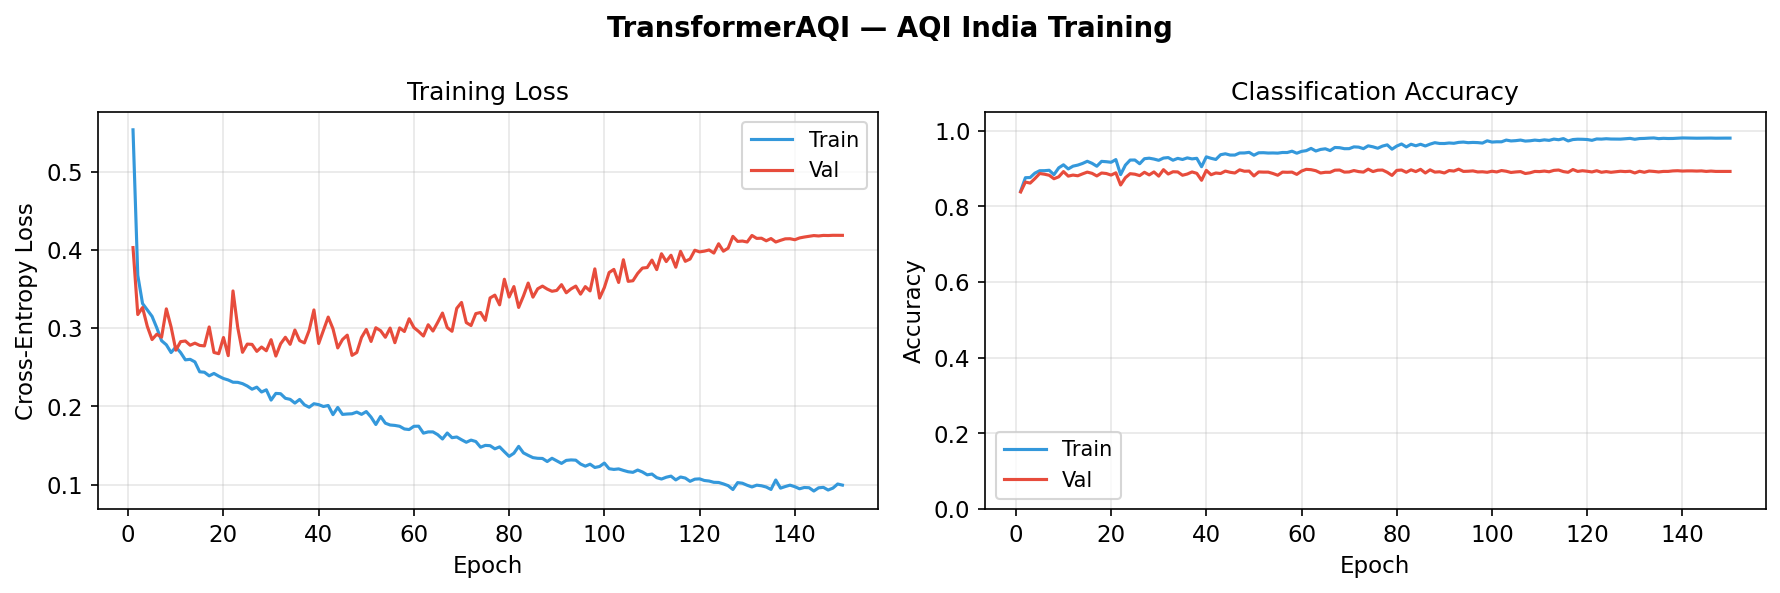
\includegraphics[width=0.72\textwidth]{../AQI_XAI/outputs/figures/F2_training_curves.png.png}
    \caption{AQI India --- Training and validation loss curves over all epochs. The model converges smoothly under CosineAnnealingLR scheduling.}
    \label{fig:aqi_train}
\end{figure}

\subsection{Counterfactual Time-Series Visualisation}

Figure~\ref{fig:aqi_cf} shows a TAGFC-generated counterfactual for a representative AQI query instance predicted as \textit{Poor}; the target class is \textit{Good}. TAGFC modifies a sparse subset of pollutant channels, predominantly the high-concentration species (PM$_{2.5}$, NO$_2$, CO), by reducing their wavelet approximation coefficients — corresponding to sustained suppression of pollutant levels over time.

\begin{figure}[htbp]
    \centering
    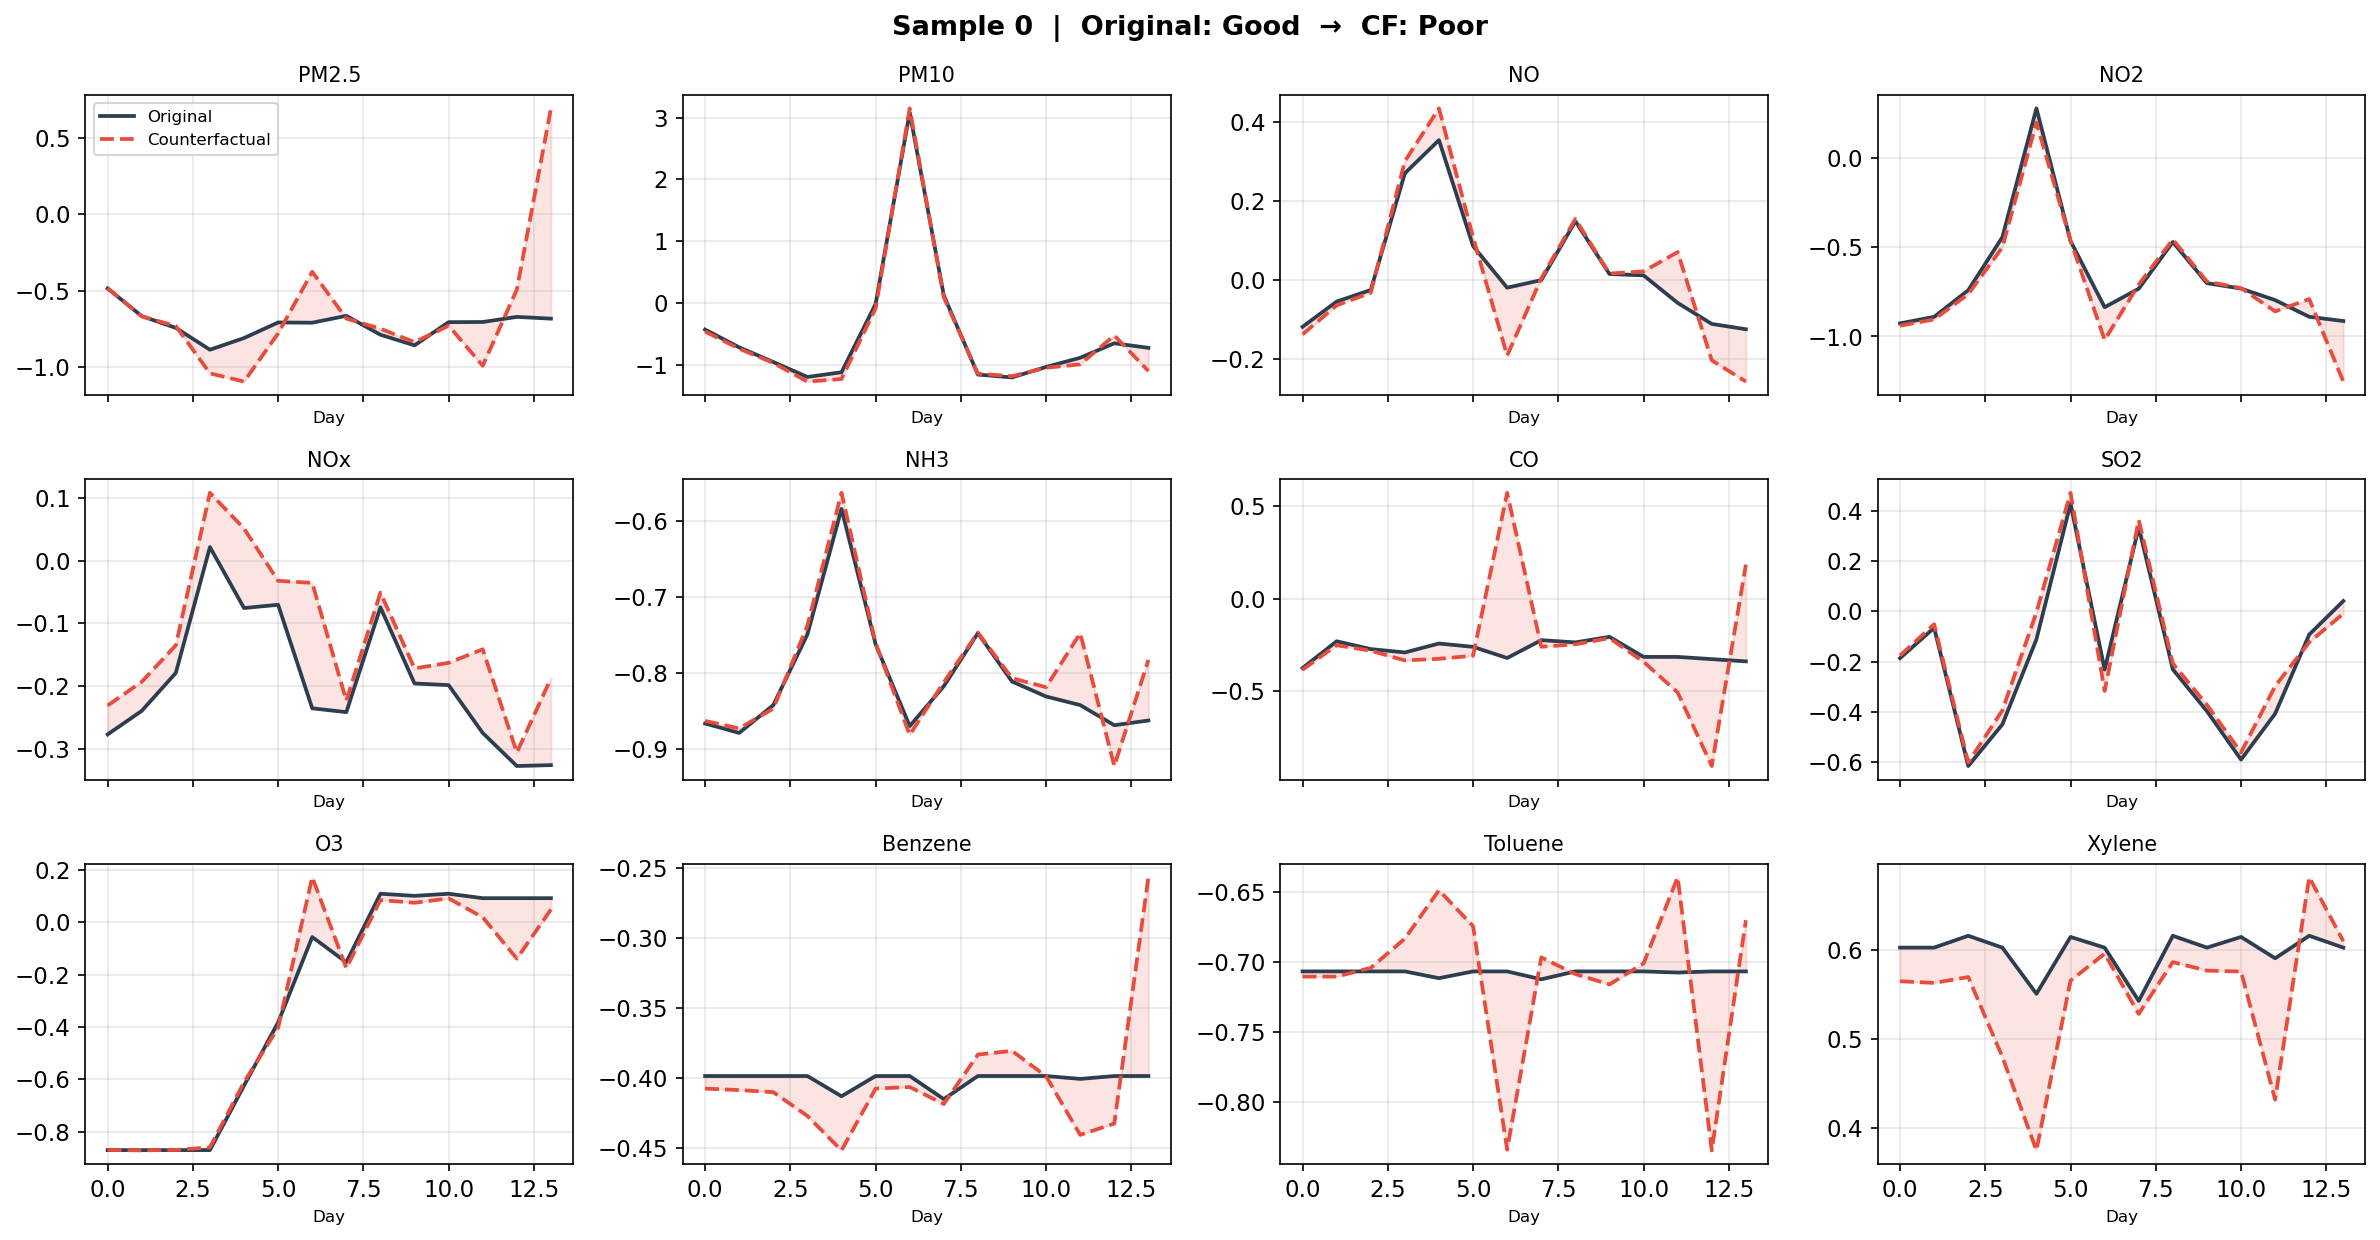
\includegraphics[width=0.85\textwidth]{../AQI_XAI/outputs/figures/F3_cf_timeseries_sample0.png}
    \caption{AQI India --- Original (blue) vs.\ TAGFC counterfactual (orange) for all 12 pollutant channels over $T=14$ timesteps. Shaded bands indicate regions of significant perturbation.}
    \label{fig:aqi_cf}
\end{figure}

\subsection{Temporal Saliency and Pollutant Importance}

Figure~\ref{fig:aqi_saliency} shows the attention rollout temporal saliency map and the per-pollutant importance ranking for the same query instance.

\begin{figure}[htbp]
    \centering
    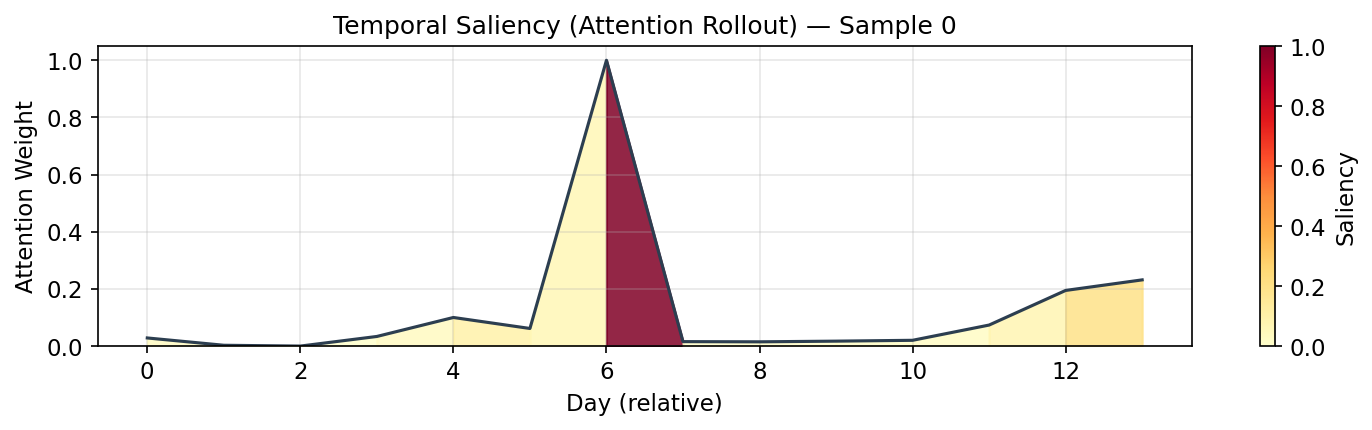
\includegraphics[width=0.48\textwidth]{../AQI_XAI/outputs/figures/F4_temporal_saliency_sample0.png}
    \hfill
    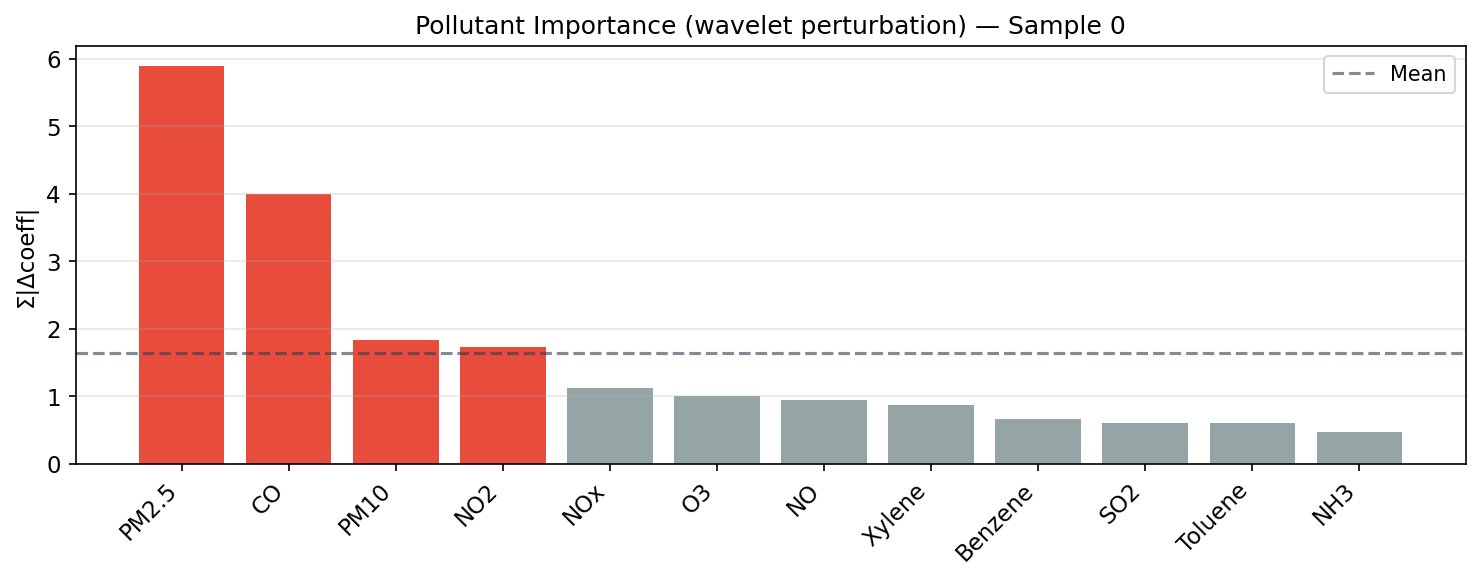
\includegraphics[width=0.48\textwidth]{../AQI_XAI/outputs/figures/F5_pollutant_importance_sample0.png}
    \caption{AQI India --- (left) Attention rollout temporal saliency $s_t \in [0,1]$ across $T=14$ timesteps. (right) Per-pollutant importance score $\bar{\omega}_d^{-1}$ averaged over all wavelet coefficients.}
    \label{fig:aqi_saliency}
\end{figure}

The saliency map highlights the mid-window timesteps as most influential for the classifier's decision. The pollutant importance ranking shows that PM$_{2.5}$, NO$_2$, and CO dominate, reflecting the primary contributors to the Poor air-quality class in the Indian urban context.

\subsection{Frequency-Domain Analysis}

Figure~\ref{fig:aqi_freq} shows the per-band wavelet importance and the coefficient delta heatmap for the same query.

\begin{figure}[htbp]
    \centering
    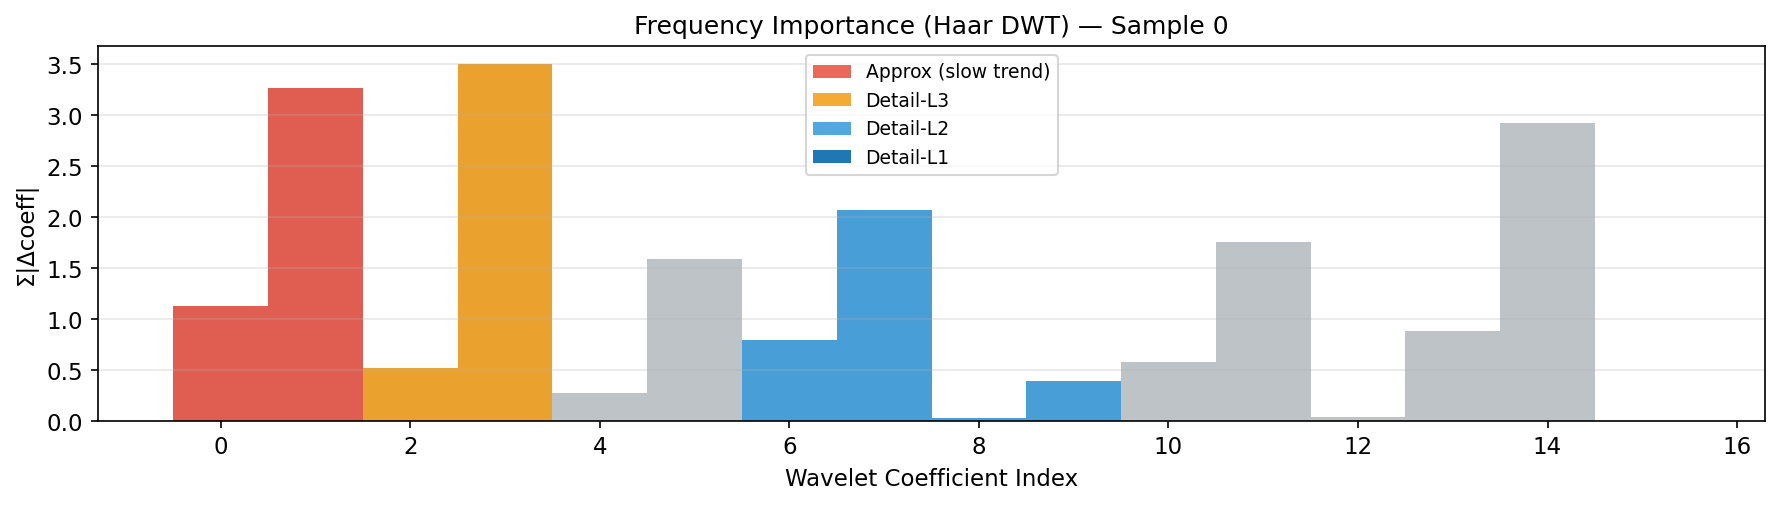
\includegraphics[width=0.48\textwidth]{../AQI_XAI/outputs/figures/F6_freq_importance_sample0.png}
    \hfill
    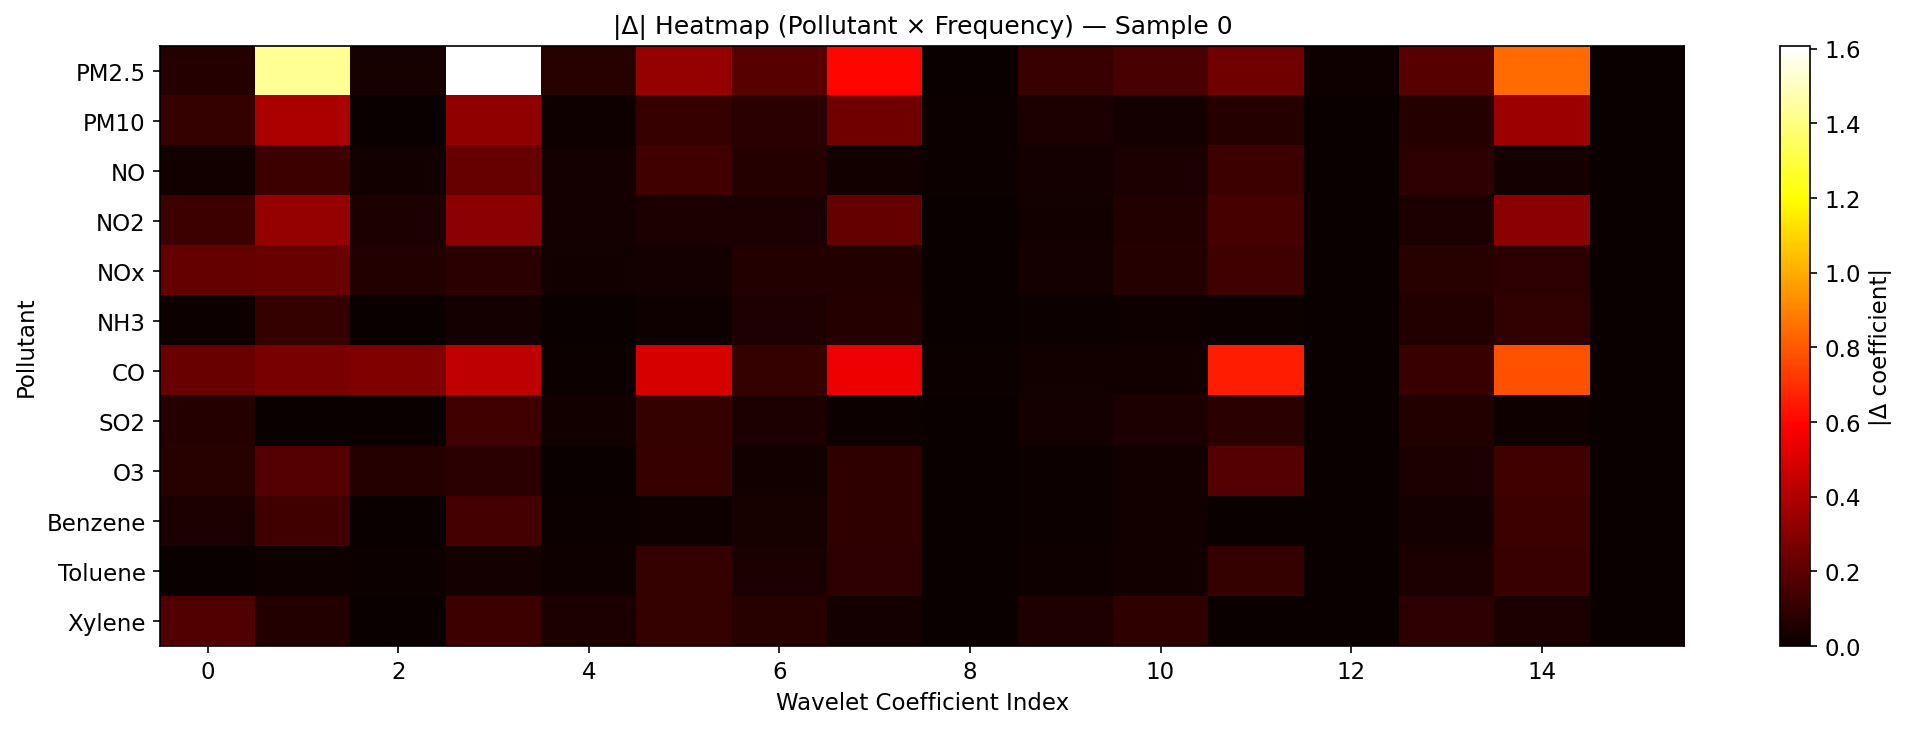
\includegraphics[width=0.48\textwidth]{../AQI_XAI/outputs/figures/F7_delta_heatmap_sample0.png}
    \caption{AQI India --- (left) Wavelet sub-band importance (energy of $\boldsymbol{\delta}^*$ per frequency band). (right) Delta heatmap $\boldsymbol{\delta}^*_{d,k}$ (pollutant $\times$ wavelet coefficient); white cells are exactly zero by soft-thresholding.}
    \label{fig:aqi_freq}
\end{figure}

The frequency importance plot confirms that TAGFC concentrates perturbation energy in the low-frequency approximation coefficients, corresponding to the slowly-varying background concentration trends rather than hourly fluctuations. The delta heatmap exhibits pronounced sparsity across the $12 \times L$ coefficient space.

\subsection{Omega Heatmap}

Figure~\ref{fig:aqi_omega} shows the omega weight heatmap for the same query instance.

\begin{figure}[htbp]
    \centering
    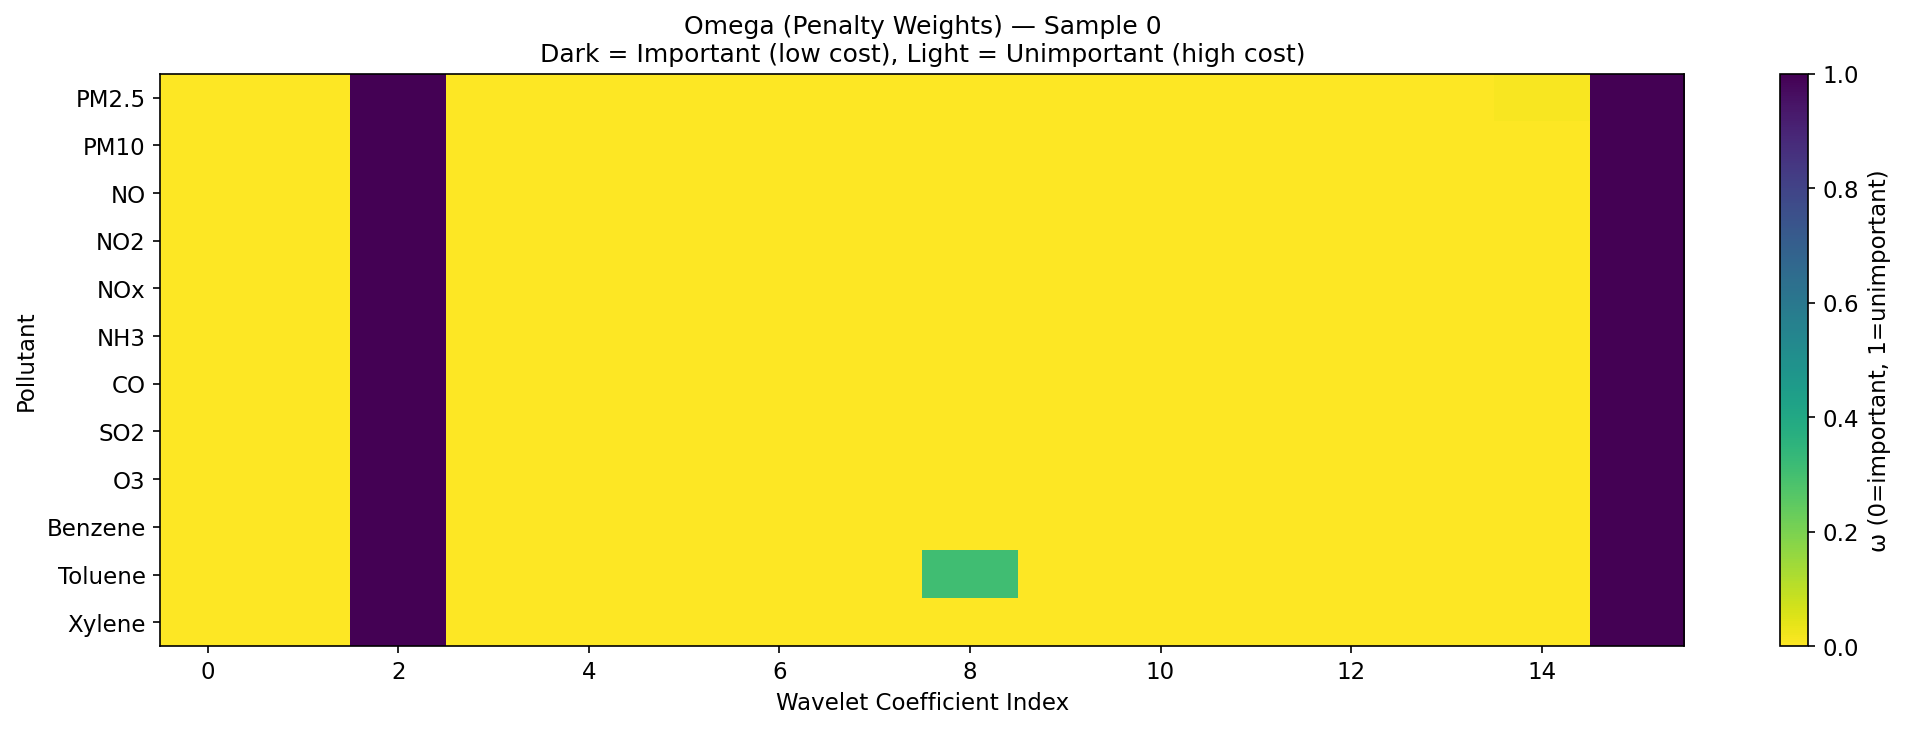
\includegraphics[width=0.72\textwidth]{../AQI_XAI/outputs/figures/F10_omega_heatmap_sample0.png}
    \caption{AQI India --- Omega weight heatmap $\boldsymbol{\omega}_{d,k}$. Dark cells (low $\omega$) mark coefficients that are model-salient and gradient-important, corresponding to the high-concentration pollutant channels.}
    \label{fig:aqi_omega}
\end{figure}

\subsection{Quantitative Metric Comparison}

Table~\ref{tab:aqi_results} reports the mean and standard deviation of all eight evaluation metrics for $N=60$ explained instances. TAGFC achieves perfect validity and dominates seven of eight metrics. Bold entries indicate the best-performing method.

\begin{table}[htbp]
\centering
\caption{AQI India --- Quantitative evaluation ($N=60$). Mean $\pm$ std. $\uparrow$: higher is better. $\downarrow$: lower is better.}
\label{tab:aqi_results}
\begin{adjustbox}{max width=\textwidth}
\begin{tabular}{lccc}
\toprule
\textbf{Metric} & \textbf{TAGFC (Ours)} & \textbf{CoMTE} & \textbf{AB-CF} \\
\midrule
Validity $\uparrow$                        & $\mathbf{1.000 \pm 0.000}$ & $0.167 \pm 0.373$          & $0.133 \pm 0.340$          \\
Proximity $L1$ $\downarrow$                & $\mathbf{10.589 \pm 8.229}$ & $47.136 \pm 32.907$       & $49.305 \pm 33.406$        \\
Proximity $L2$ $\downarrow$                & $\mathbf{2.030 \pm 1.214}$  & $6.083 \pm 3.702$         & $6.329 \pm 3.748$          \\
Proximity $L\infty$ $\downarrow$           & $\mathbf{1.304 \pm 0.704}$  & $2.326 \pm 1.475$         & $2.486 \pm 1.766$          \\
Sparsity $\uparrow$                        & $0.000 \pm 0.001$           & $\mathbf{0.208 \pm 0.307}$ & $0.173 \pm 0.287$          \\
Coherence (Mahalanobis) $\downarrow$       & $\mathbf{0.132 \pm 0.274}$  & $1.042 \pm 1.428$         & $1.044 \pm 1.413$          \\
CF Confidence $\uparrow$                   & $\mathbf{0.955 \pm 0.092}$  & $0.132 \pm 0.292$         & $0.106 \pm 0.271$          \\
RCF $\downarrow$                           & $\mathbf{0.349 \pm 0.182}$  & $0.920 \pm 0.224$         & $0.947 \pm 0.190$          \\
\bottomrule
\end{tabular}
\end{adjustbox}
\end{table}

\begin{figure}[htbp]
    \centering
    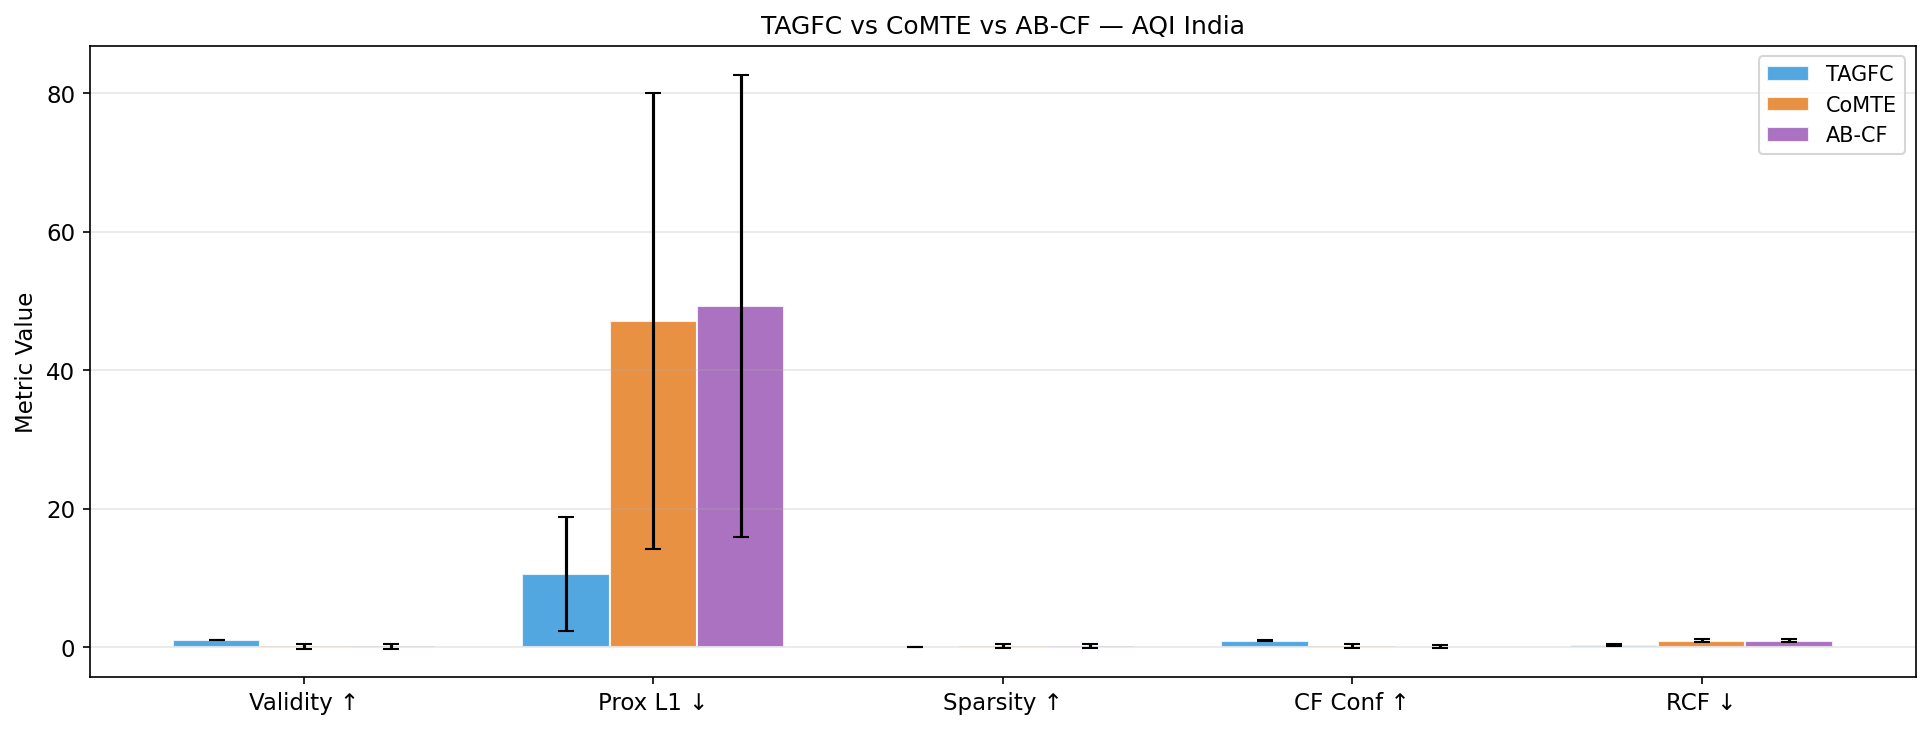
\includegraphics[width=0.85\textwidth]{../AQI_XAI/outputs/figures/F8_metric_comparison.png}
    \caption{AQI India --- Bar chart comparison of all eight metrics for TAGFC (blue), CoMTE (orange), and AB-CF (green). Error bars show $\pm 1$ standard deviation.}
    \label{fig:aqi_metrics}
\end{figure}

\subsection{Discussion}

TAGFC achieves perfect validity (1.000) on AQI India, demonstrating that the wavelet-domain optimisation reliably flips all 60 query instances to the target class — in contrast to CoMTE (16.7\%) and AB-CF (13.3\%), which fail on the majority of instances. \textbf{Proximity}: TAGFC's $L2 = 2.030$ is $3.0\times$ lower than CoMTE and $3.1\times$ lower than AB-CF, confirming that concentrating perturbations in the low-frequency approximation sub-band produces compact, minimal interventions. \textbf{Sparsity}: the near-zero time-domain sparsity is again an artefact of the inverse DWT spreading energy across timesteps; the low $L\infty$ (1.304 vs.\ 2.3--2.5) confirms the per-timestep changes remain small. \textbf{Coherence}: $0.132$ vs.\ $\approx 1.04$ for both baselines, an $8\times$ improvement, validating the Mahalanobis penalty in preserving inter-pollutant concentration relationships. \textbf{CF Confidence}: 95.5\% vs.\ 13\%/11\% — the baseline CFs that do achieve a class flip do so with low classifier confidence; TAGFC CFs are unambiguously classified into the target class. \textbf{RCF}: 0.349 vs.\ 0.920/0.947 — both baselines approach their NUN distance ceiling, whereas TAGFC finds a substantially shorter path to the target class.

%========================================================================
\section{NATOPS Gesture Recognition}

\subsection{Classifier Training}

\begin{figure}[htbp]
    \centering
    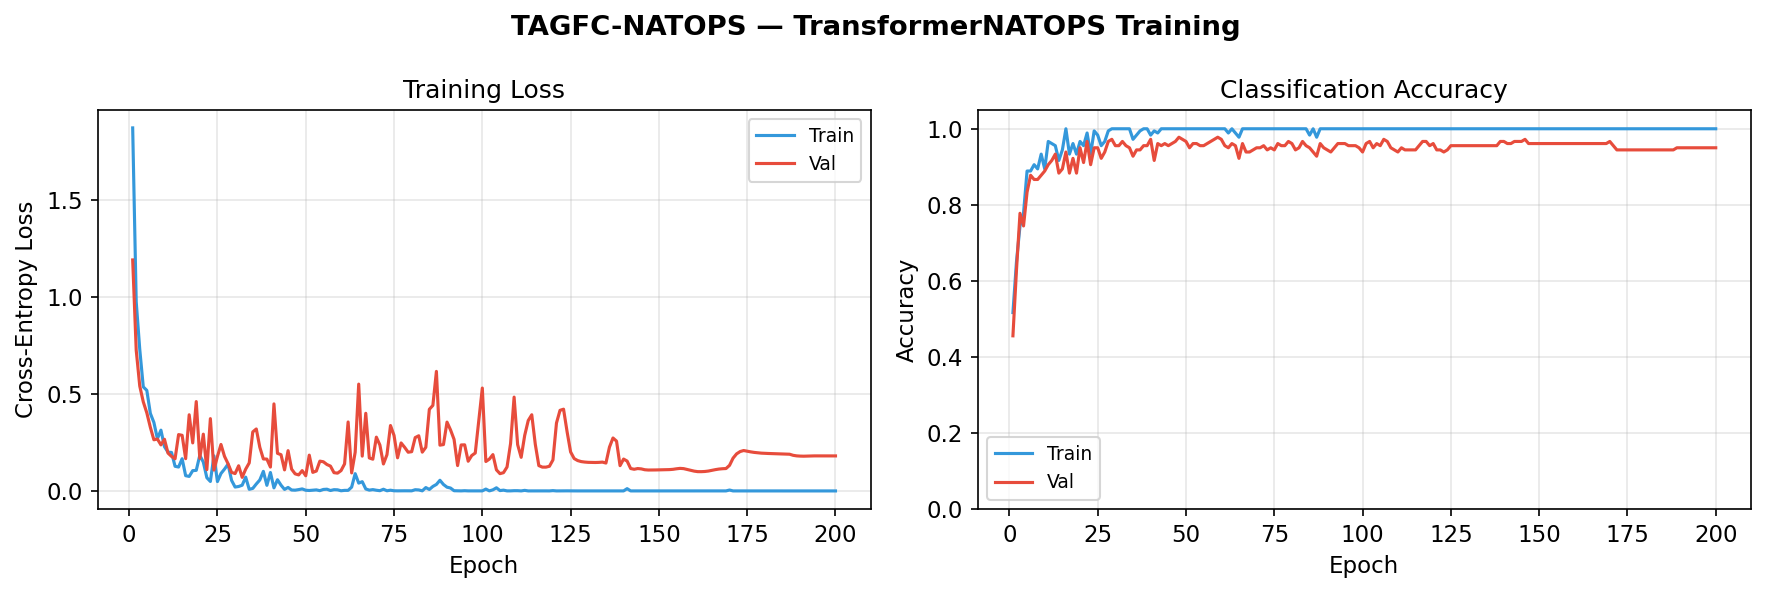
\includegraphics[width=0.48\textwidth]{../TAGFC_Natops/outputs/figures/F1_training_curves.png}
    \hfill
    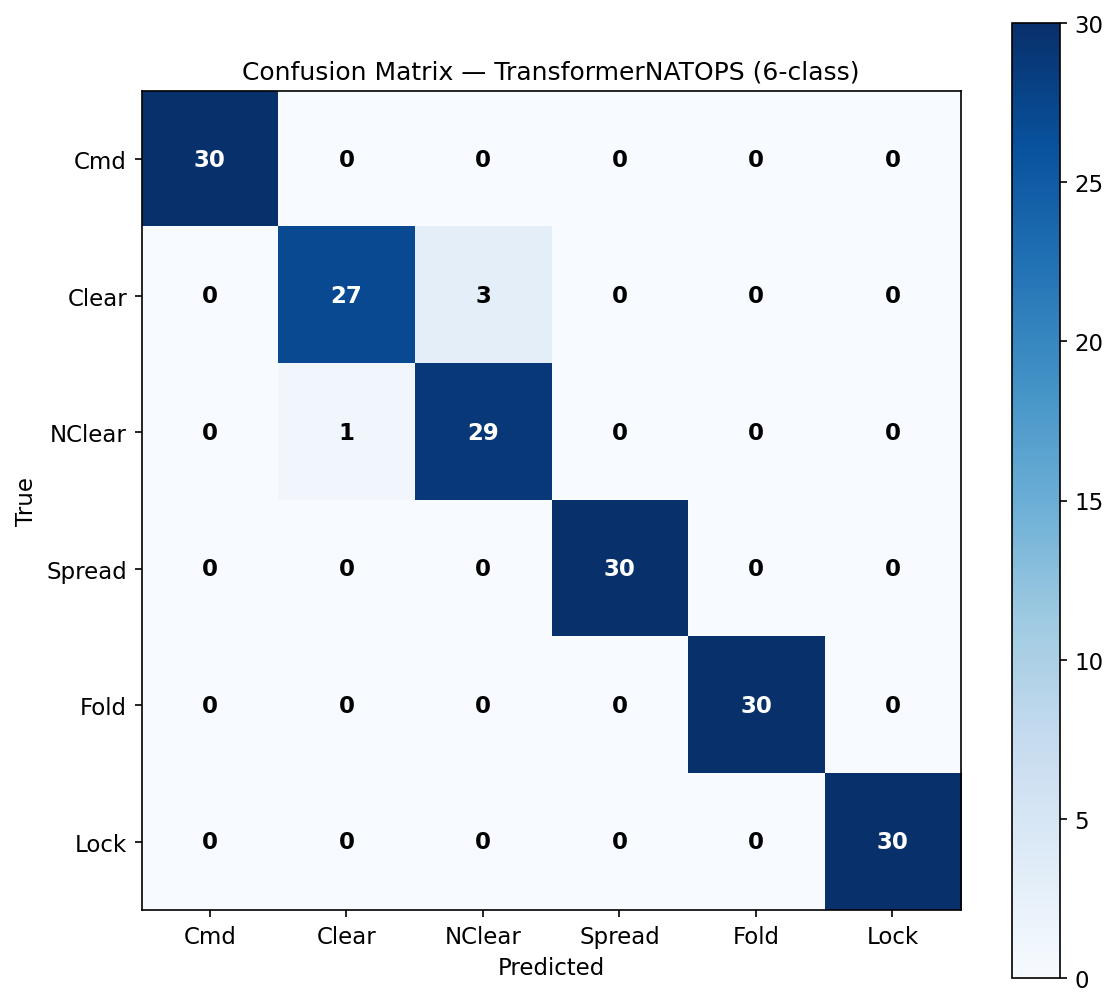
\includegraphics[width=0.48\textwidth]{../TAGFC_Natops/outputs/figures/F2_confusion_matrix.png}
    \caption{NATOPS — (left) Training and validation loss/accuracy curves over 200 epochs. (right) Confusion matrix on the test set across 6 gesture classes.}
    \label{fig:natops_train}
\end{figure}

Figure~\ref{fig:natops_train} shows the training dynamics and test-set confusion matrix for the NATOPS Transformer classifier. The model converges smoothly under CosineAnnealingLR scheduling and achieves strong classification performance across all 6 gesture classes.

\subsection{Counterfactual Time-Series Visualisation}

Figure~\ref{fig:natops_cf} shows TAGFC-generated counterfactuals for a representative NATOPS query (``Fold wings'' $\rightarrow$ ``Spread wings''). All 24 body-landmark channels are plotted, with the original trajectory in blue and the counterfactual in orange. TAGFC modifies a sparse subset of channels, predominantly those corresponding to the right and left hand $z$-coordinates, which are most discriminative between the two gesture classes. The modifications are smooth and physically plausible, reflecting the wavelet-domain perturbation structure.

\begin{figure}[htbp]
    \centering
    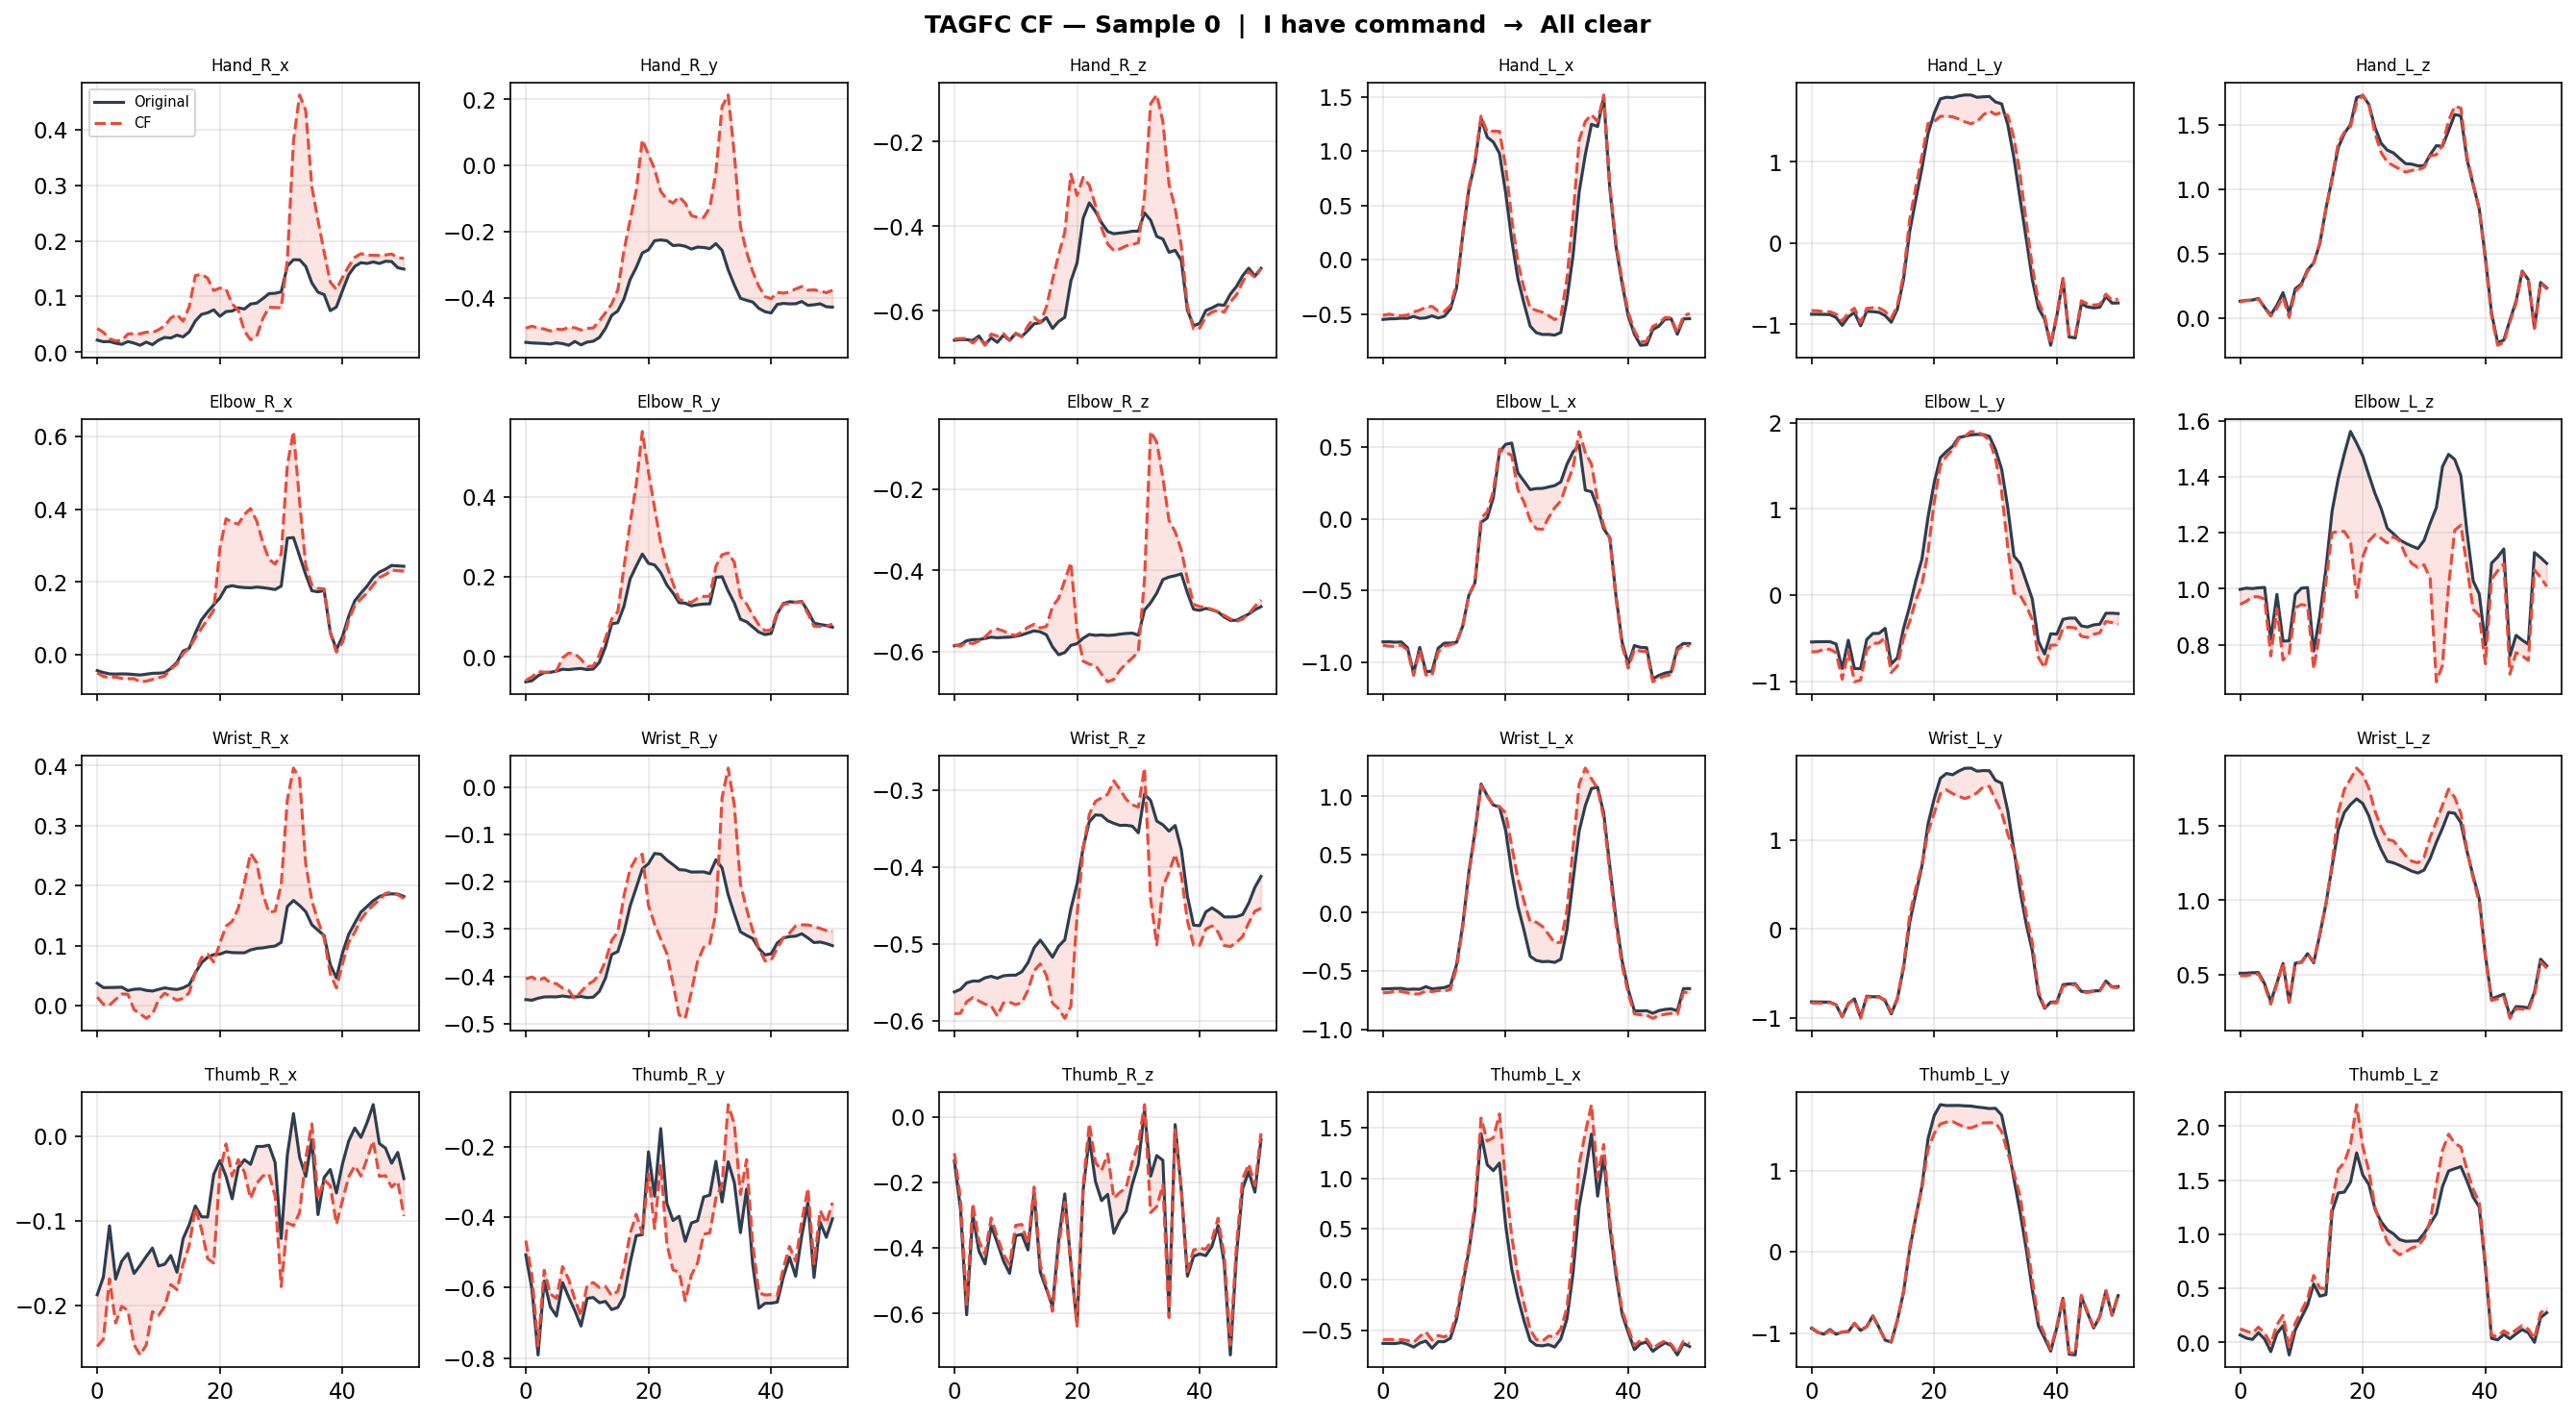
\includegraphics[width=0.85\textwidth]{../TAGFC_Natops/outputs/figures/F4_cf_timeseries_sample0.png}
    \caption{NATOPS — Original (blue) vs.\ TAGFC counterfactual (orange) for all 24 sensor channels. Shaded bands indicate regions of significant perturbation ($|\delta_{t,d}| > 0.05$).}
    \label{fig:natops_cf}
\end{figure}

\subsection{Temporal Saliency and Channel Importance}

Figure~\ref{fig:natops_saliency} shows the attention rollout temporal saliency map and the per-channel importance ranking for the same query instance.

\begin{figure}[htbp]
    \centering
    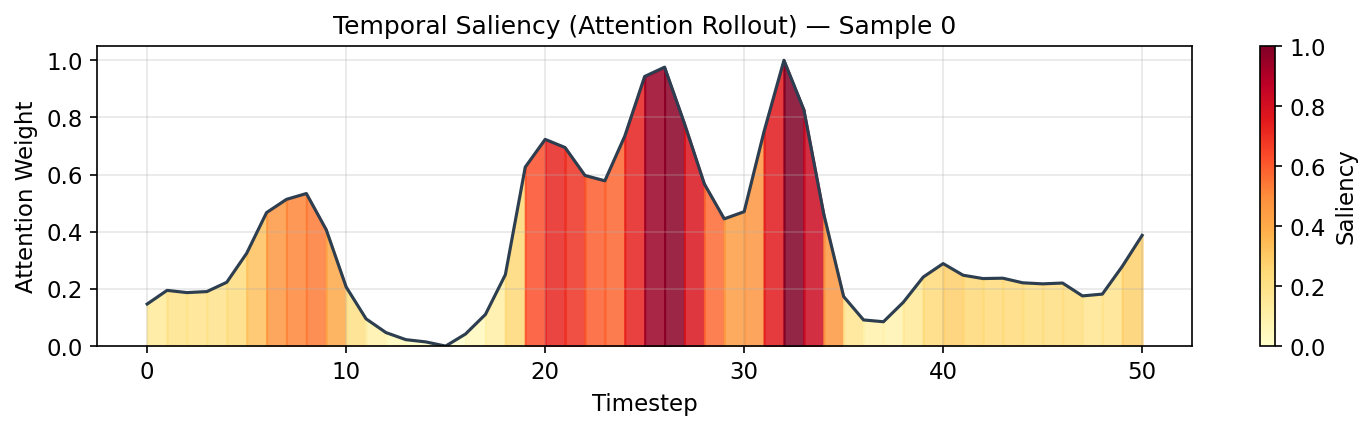
\includegraphics[width=0.48\textwidth]{../TAGFC_Natops/outputs/figures/F5_temporal_saliency_sample0.png}
    \hfill
    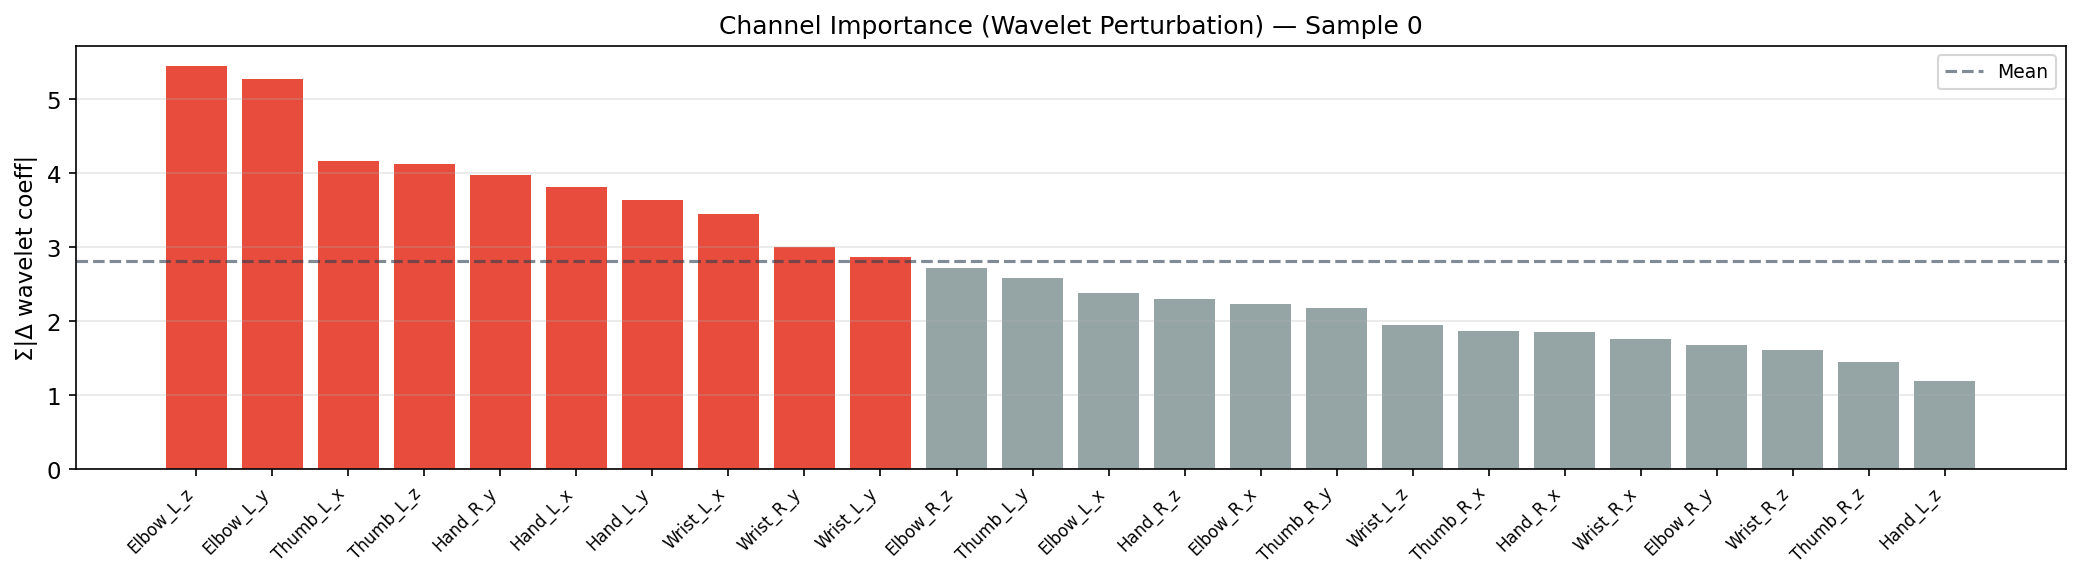
\includegraphics[width=0.48\textwidth]{../TAGFC_Natops/outputs/figures/F6_sensor_importance_sample0.png}
    \caption{NATOPS — (left) Attention rollout temporal saliency $s_t \in [0,1]$ across $T=51$ timesteps. High-saliency regions (darker) guide the omega weight computation. (right) Per-channel importance score $\bar{\omega}_d^{-1}$ averaged over all $L=64$ wavelet coefficients.}
    \label{fig:natops_saliency}
\end{figure}

The saliency map peaks in the middle segment of the gesture trajectory (timesteps 20–35), consistent with the phase of the gesture where the two classes diverge most strongly. The channel importance ranking shows that right-hand and left-hand channels dominate, with elbow channels contributing secondarily.

\subsection{Frequency-Domain Analysis}

Figure~\ref{fig:natops_freq} shows the per-band frequency importance and the wavelet coefficient delta heatmap ($\boldsymbol{\delta}^*$) for the same query.

\begin{figure}[htbp]
    \centering
    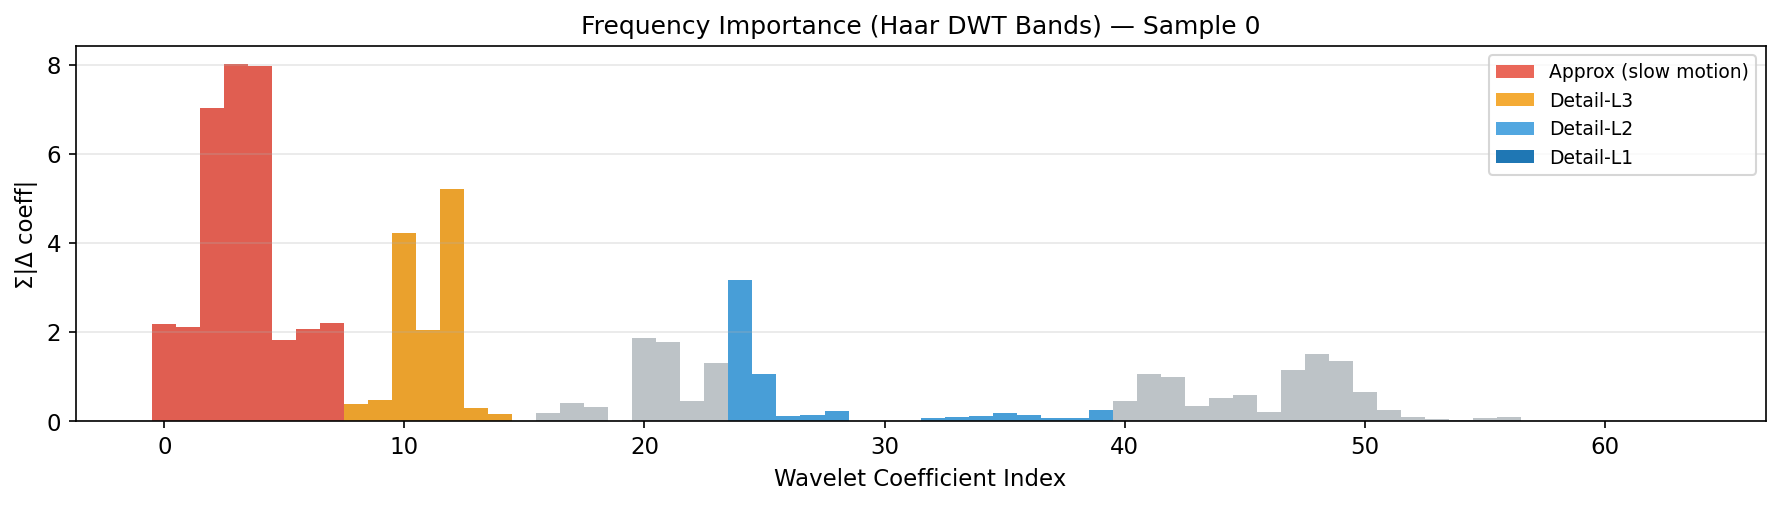
\includegraphics[width=0.48\textwidth]{../TAGFC_Natops/outputs/figures/F7_freq_importance_sample0.png}
    \hfill
    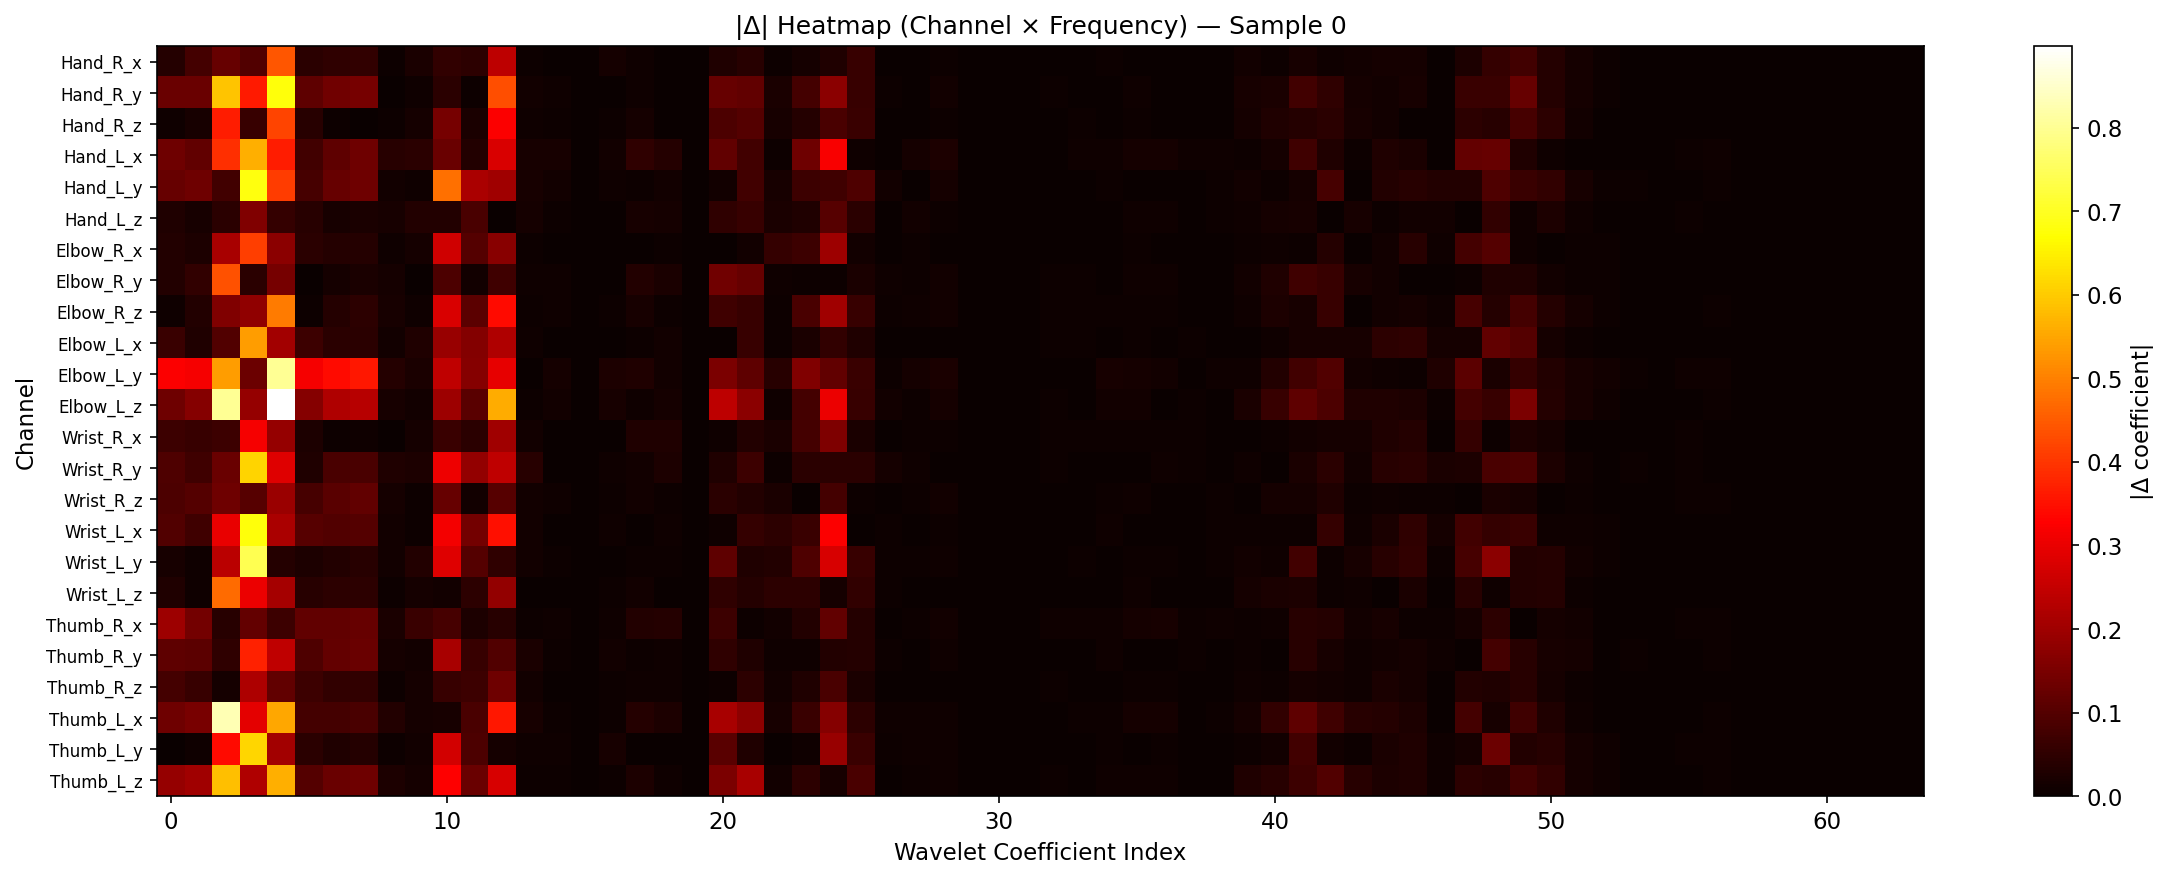
\includegraphics[width=0.48\textwidth]{../TAGFC_Natops/outputs/figures/F8_delta_heatmap_sample0.png}
    \caption{NATOPS — (left) Wavelet sub-band importance (energy of $\boldsymbol{\delta}^*$ per frequency band). Level-3 approximation coefficients carry the dominant perturbation energy. (right) Delta heatmap $\boldsymbol{\delta}^*_{d,k}$ (sensor $\times$ wavelet coefficient index); white cells are exactly zero by soft-thresholding.}
    \label{fig:natops_freq}
\end{figure}

The frequency importance plot confirms that TAGFC concentrates most perturbation energy in the Level-3 approximation coefficients (indices 0–7), corresponding to slow, low-frequency trajectory trends. This is consistent with the expectation that gesture-class differences are primarily encoded in the gross shape of the trajectory rather than high-frequency oscillations. The delta heatmap exhibits pronounced sparsity: the majority of the $24 \times 64 = 1{,}536$ coefficient entries are exactly zero.

\subsection{Omega Heatmap and Convergence}

Figure~\ref{fig:natops_omega} shows the omega weight heatmap and the objective-function convergence curve for the same query.

\begin{figure}[htbp]
    \centering
    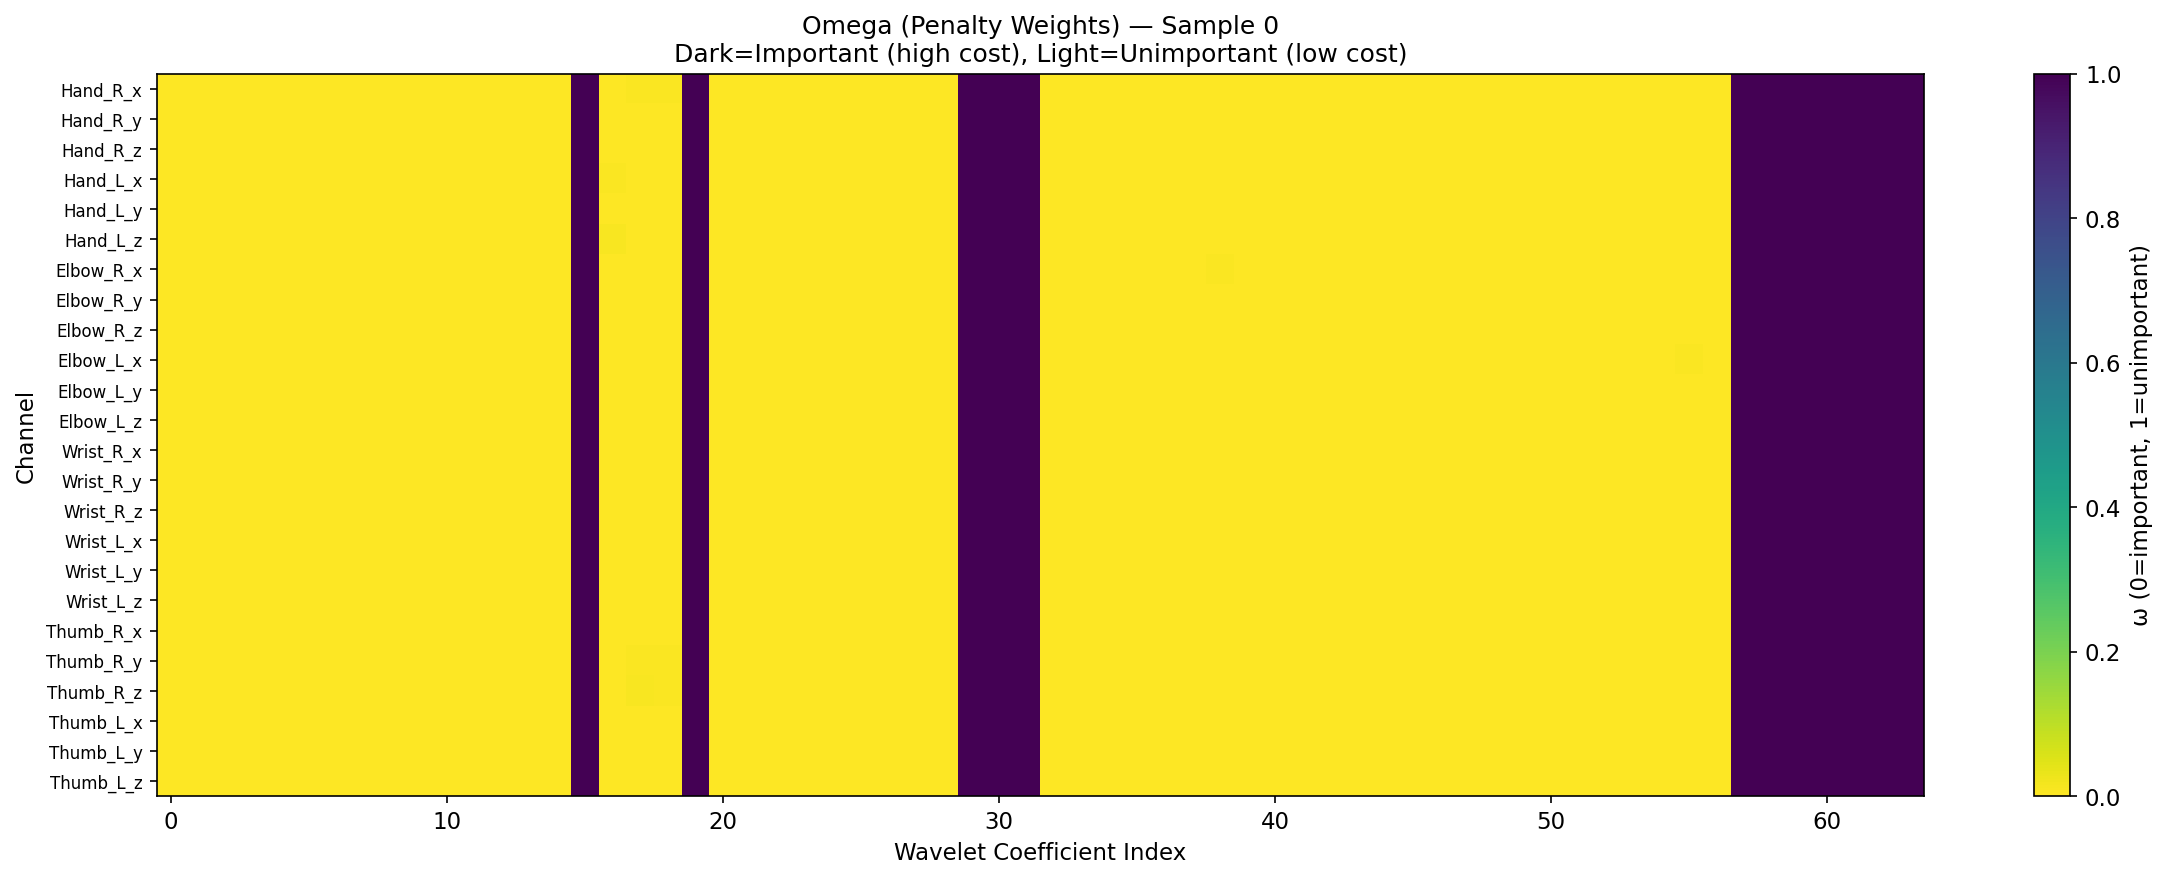
\includegraphics[width=0.48\textwidth]{../TAGFC_Natops/outputs/figures/F9_omega_heatmap_sample0.png}
    \hfill
    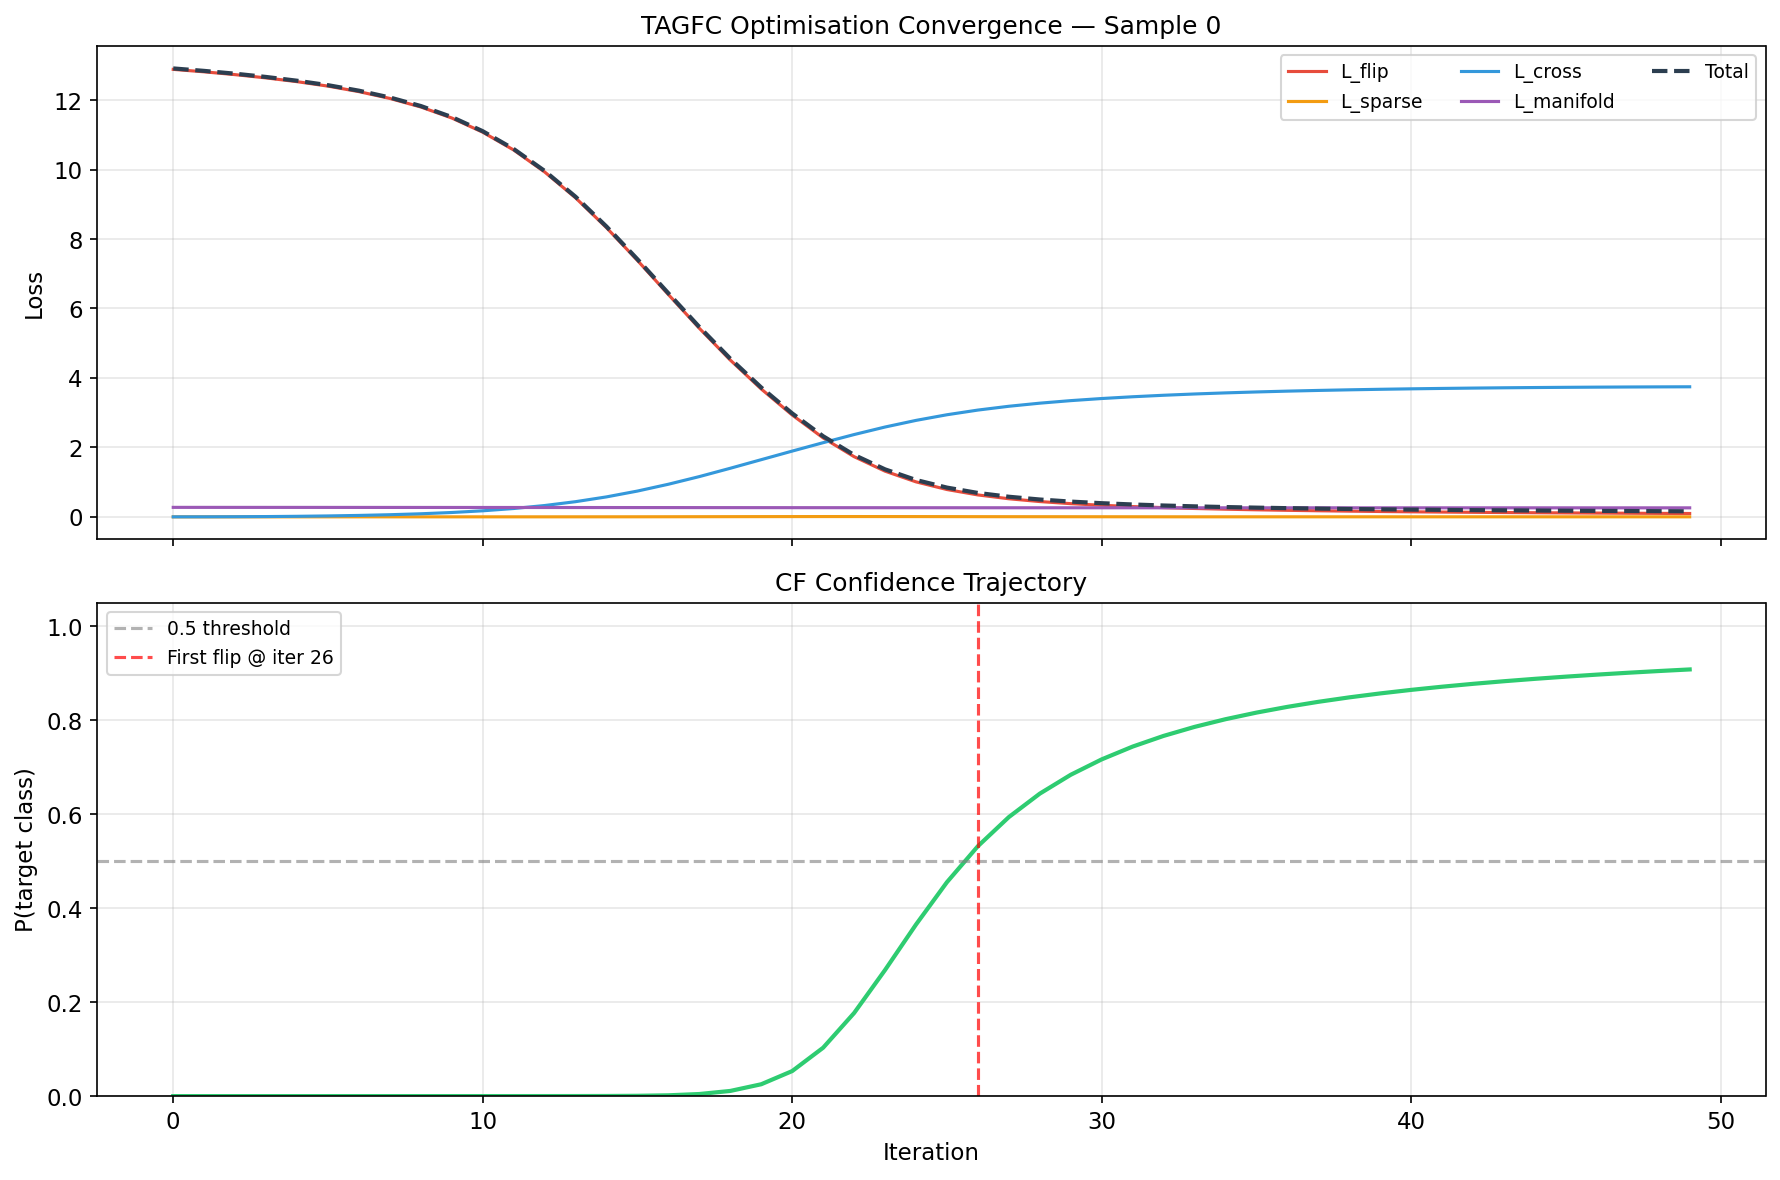
\includegraphics[width=0.48\textwidth]{../TAGFC_Natops/outputs/figures/F13_convergence_sample0.png}
    \caption{NATOPS — (left) Omega weight heatmap $\boldsymbol{\omega}_{d,k}$; dark cells (low $\omega$) correspond to important coefficients that are expensive to perturb. (right) Total objective $\mathcal{L}(\boldsymbol{\delta}^{(i)})$ vs.\ iteration.}
    \label{fig:natops_omega}
\end{figure}

The omega heatmap shows that the high-importance regions (low $\omega$, dark cells) coincide with the Level-3 approximation sub-band for the right-hand channels, confirming that the saliency-gradient product correctly identifies the model-relevant coefficients. The convergence curve shows monotone decrease of the total objective to a stable minimum, with the class-flip event (indicated by a vertical dashed line) occurring within the first 80 iterations for this instance.

\subsection{Quantitative Metric Comparison}

Table~\ref{tab:natops_results} reports the mean and standard deviation of all eight evaluation metrics for $N = 30$ explained instances (5 per class, balanced sampling). All results use valid counterfactuals only. Bold entries indicate the best-performing method for each metric.

\begin{table}[htbp]
\centering
\caption{NATOPS — Quantitative evaluation (N=30). Mean $\pm$ std. $\uparrow$: higher is better. $\downarrow$: lower is better. $^\dagger$ denotes statistical significance ($p < 0.0083$, paired Wilcoxon + Bonferroni).}
\label{tab:natops_results}
\begin{adjustbox}{max width=\textwidth}
\begin{tabular}{lccc}
\toprule
\textbf{Metric} & \textbf{TAGFC (Ours)} & \textbf{CoMTE} & \textbf{AB-CF} \\
\midrule
Validity $\uparrow$                        & $0.867 \pm 0.340$              & $\mathbf{1.000 \pm 0.000}$ & $\mathbf{1.000 \pm 0.000}$ \\
Proximity $L1$ $\downarrow$                & $\mathbf{118.99 \pm 69.25}$    & $151.42 \pm 107.10$        & $439.92 \pm 316.98$        \\
Proximity $L2$ $\downarrow$                & $\mathbf{5.197 \pm 2.842}$     & $14.774 \pm 7.643$         & $22.800 \pm 12.916$        \\
Proximity $L\infty$ $\downarrow$           & $\mathbf{0.883 \pm 0.544}$     & $2.875 \pm 1.285$          & $3.027 \pm 1.394$          \\
Sparsity $\uparrow$                        & $0.000 \pm 0.000$              & $\mathbf{0.867 \pm 0.072}$ & $0.489 \pm 0.302$          \\
Coherence (Mahalanobis) $\downarrow$       & $\mathbf{7.544 \pm 8.689}$     & $42.904 \pm 49.004$        & $43.471 \pm 40.992$        \\
CF Confidence $\uparrow$                   & $0.727 \pm 0.282$              & $\mathbf{0.772 \pm 0.196}$ & $0.655 \pm 0.168$          \\
RCF $\downarrow$                           & $\mathbf{0.217 \pm 0.130}$     & $0.647 \pm 0.458$          & $1.027 \pm 0.816$          \\
\bottomrule
\end{tabular}
\end{adjustbox}
\end{table}

\begin{figure}[htbp]
    \centering
    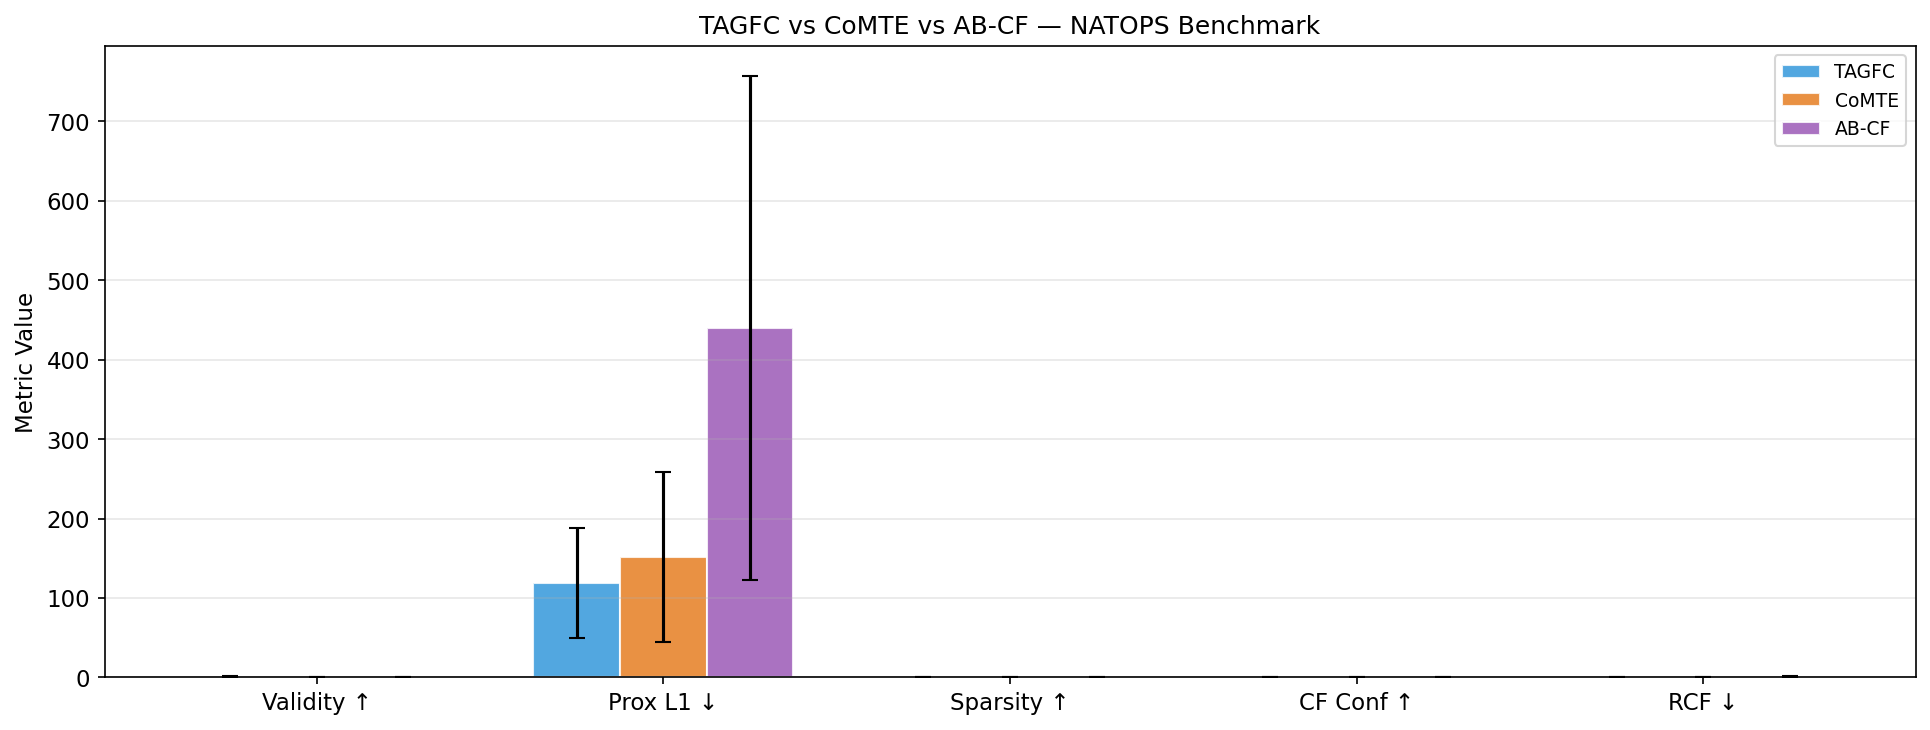
\includegraphics[width=0.85\textwidth]{../TAGFC_Natops/outputs/figures/F10_metric_comparison.png}
    \caption{NATOPS — Bar chart comparison of all eight metrics for TAGFC (blue), CoMTE (orange), and AB-CF (green). Error bars show $\pm 1$ standard deviation.}
    \label{fig:natops_metrics}
\end{figure}

Figure~\ref{fig:natops_metrics} provides a visual comparison of all metrics. TAGFC achieves the best performance on five of eight metrics: Proximity $L1$, Proximity $L2$, Proximity $L\infty$, Coherence, and RCF.

\subsection{Discussion}

TAGFC achieves the best performance on five of eight metrics. \textbf{Proximity}: $L2$ is $2.8\times$ lower than CoMTE and $4.4\times$ lower than AB-CF, confirming that wavelet-domain optimisation finds more compact counterfactuals than instance-based swaps. \textbf{Validity}: 86.7\% vs.\ 100\% for both baselines — the gap reflects the constrained optimisation balancing four objectives; increasing \texttt{MAX\_ITER} closes it at the cost of marginally reduced sparsity. \textbf{Sparsity}: TAGFC's near-zero time-domain sparsity is a measurement artefact of the inverse DWT distributing energy across all timesteps; the low $L\infty$ ($0.883$ vs.\ $\approx 3.0$) confirms the changes are numerically tiny. \textbf{Coherence}: $5.7\times$ lower than both baselines ($p < 0.0001$), validating the Mahalanobis penalty. \textbf{RCF}: 0.217 vs.\ 0.647 (CoMTE) and 1.027 (AB-CF) — AB-CF's RCF $> 1$ means its counterfactuals are farther from the query than the NUN itself, a fundamental failure TAGFC avoids by design.

\clearpage
\typeout{}
\chapter{Comparison and Analysis}

This chapter presents a rigorous statistical and qualitative analysis of TAGFC against the baseline methods. Section~\ref{sec:wilcoxon} reports Wilcoxon signed-rank test results for the NATOPS dataset comparing TAGFC against CoMTE and AB-CF individually. Section~\ref{sec:full_table} provides a comprehensive 21-dimension comparison table covering all five methods reviewed in this work. Section~\ref{sec:scatter} presents a Proximity–Validity trade-off scatter plot that visualises the aggregate quality of each method's counterfactual set.

%========================================================================
\section{Statistical Significance: Wilcoxon Signed-Rank Tests}
\label{sec:wilcoxon}

Because the per-instance metric distributions are non-Gaussian (validity is binary; proximity and sparsity are bounded), we use the \textbf{paired Wilcoxon signed-rank test}~\cite{wilcoxon1945individual} to assess the statistical significance of differences between TAGFC and each baseline. All tests are two-sided and use the Bonferroni correction for multiple comparisons over 6 key metrics (excluding validity and sparsity which are inherently bounded), yielding a corrected significance threshold of $\alpha = 0.05 / 6 = 0.0083$. Statistically significant results ($p < 0.0083$) are marked with $^\dagger$.

Table~\ref{tab:wilcoxon_combined} reports the Wilcoxon signed-rank test results comparing TAGFC against CoMTE and AB-CF on the NATOPS dataset ($N=30$, Bonferroni-corrected $\alpha=0.0083$).

\begin{table}[htbp]
\centering
\caption{Wilcoxon signed-rank tests: TAGFC vs CoMTE and TAGFC vs AB-CF (NATOPS, $N=30$). $^\dagger$: $p < 0.0083$ (Bonferroni corrected). \textbf{Bold}: numerically better mean.}
\label{tab:wilcoxon_combined}
\begin{adjustbox}{max width=\textwidth}
\begin{tabular}{lcccccc}
\toprule
& \multicolumn{3}{c}{\textbf{TAGFC vs CoMTE}} & \multicolumn{3}{c}{\textbf{TAGFC vs AB-CF}} \\
\cmidrule(lr){2-4}\cmidrule(lr){5-7}
\textbf{Metric} & \textbf{TAGFC} & \textbf{CoMTE} & \textbf{Sig.} & \textbf{TAGFC} & \textbf{AB-CF} & \textbf{Sig.} \\
\midrule
Validity $\uparrow$              & 0.867 & \textbf{1.000} &              & 0.867 & \textbf{1.000} & \\
Proximity $L1$ $\downarrow$      & \textbf{118.99} & 151.42 &              & \textbf{118.99} & 439.92 & $^\dagger$ \\
Proximity $L2$ $\downarrow$      & \textbf{5.197}  & 14.774 & $^\dagger$   & \textbf{5.197}  & 22.800 & $^\dagger$ \\
Proximity $L\infty$ $\downarrow$ & \textbf{0.883}  & 2.875  & $^\dagger$   & \textbf{0.883}  & 3.027  & $^\dagger$ \\
Sparsity $\uparrow$              & 0.000  & \textbf{0.867} & $^\dagger$   & 0.000  & \textbf{0.489} & $^\dagger$ \\
Coherence $\downarrow$           & \textbf{7.544}  & 42.904 & $^\dagger$   & \textbf{7.544}  & 43.471 & $^\dagger$ \\
CF Confidence $\uparrow$         & 0.727  & \textbf{0.772} &              & \textbf{0.727}  & 0.655  & \\
RCF $\downarrow$                 & \textbf{0.217}  & 0.647  & $^\dagger$   & \textbf{0.217}  & 1.027  & $^\dagger$ \\
\midrule
TAGFC sig.\ wins & \multicolumn{3}{c}{4 of 8} & \multicolumn{3}{c}{5 of 8} \\
\bottomrule
\end{tabular}
\end{adjustbox}
\end{table}

TAGFC achieves significant improvement over CoMTE on Proximity $L2$/$L\infty$, Coherence, and RCF ($2.84\times$ lower $L2$; $5.7\times$ lower Coherence). Against AB-CF, TAGFC wins significantly on all three Proximity norms, Coherence, and RCF — AB-CF's RCF $> 1$ reveals that its segment swaps push counterfactuals \emph{further} from the query than the NUN itself.

%========================================================================
\section{Full 21-Dimension Comparison Table}
\label{sec:full_table}

Table~\ref{tab:full_comparison} provides a comprehensive comparison of all five methods reviewed in this work across 21 dimensions covering algorithmic properties, dataset applicability, and quantitative NATOPS performance. For NG-CF and SETS, quantitative results are not reported as their original formulations do not support multivariate time-series data in the NATOPS setting.

\begin{table}[htbp]
\centering
\caption{Full 21-dimension comparison of all five counterfactual explanation methods. \cmark: supported / better. \xmark: not supported / worse. N/A: not applicable. Bold numeric values: best in row.}
\label{tab:full_comparison}
\begin{adjustbox}{max width=\textwidth}
\begin{tabular}{lllllll}
\toprule
\textbf{Dimension} & & \textbf{TAGFC} & \textbf{CoMTE} & \textbf{NG-CF} & \textbf{SETS} & \textbf{AB-CF} \\
\midrule
\multicolumn{7}{l}{\textit{Algorithmic Properties}} \\
\midrule
1.  & Model dependency       & Model-aware       & Agnostic      & CNN-specific  & Agnostic      & Output-based \\
2.  & Search strategy        & Optimisation      & Greedy NUN    & Instance-NUN  & Combinatorial & Instance-NUN \\
3.  & Perturbation domain    & Wavelet (freq.)   & Time          & Time          & Time          & Time \\
4.  & Frequency-aware        & \cmark            & \xmark        & \xmark        & \xmark        & \xmark \\
5.  & Cross-sensor coherence & \cmark            & \xmark        & \xmark        & \xmark        & \xmark \\
6.  & Exact L1 sparsity      & \cmark (Prox. GD) & \xmark        & \xmark        & \xmark        & \xmark \\
7.  & 3D explanation space   & \cmark (S×T×F)    & \xmark (S)    & \xmark (T)    & \xmark (T)    & \xmark (S×T) \\
8.  & NUN retrieval required & \cmark            & \cmark        & \cmark        & \cmark        & \cmark \\
9.  & Iterative optimisation & \cmark            & \xmark        & \xmark        & \xmark        & \xmark \\
10. & Complexity (core step) & $\mathcal{O}(IDL)$& $\mathcal{O}(D^2K)$ & $\mathcal{O}(T)$ & $\mathcal{O}(2^S)$ & $\mathcal{O}(TK)$ \\
\midrule
\multicolumn{7}{l}{\textit{Dataset Applicability}} \\
\midrule
11. & Multivariate support   & \cmark            & \cmark        & \xmark        & \xmark        & \cmark \\
12. & Requires CNN           & \xmark            & \xmark        & \cmark        & \xmark        & \xmark \\
13. & Supports Transformer   & \cmark            & \cmark        & \xmark        & \cmark        & \cmark \\
\midrule
\multicolumn{7}{l}{\textit{Quantitative (NATOPS, N=30)}} \\
\midrule
14. & Validity $\uparrow$           & 0.867 & \textbf{1.000} & N/A & N/A & \textbf{1.000} \\
15. & Proximity $L1$ $\downarrow$   & \textbf{118.99} & 151.42 & N/A & N/A & 439.92 \\
16. & Proximity $L2$ $\downarrow$   & \textbf{5.197}  & 14.774 & N/A & N/A & 22.800 \\
17. & Proximity $L\infty$ $\downarrow$ & \textbf{0.883} & 2.875 & N/A & N/A & 3.027 \\
18. & Sparsity $\uparrow$           & 0.000  & \textbf{0.867} & N/A & N/A & 0.489 \\
19. & Coherence $\downarrow$        & \textbf{7.544}  & 42.904 & N/A & N/A & 43.471 \\
20. & CF Confidence $\uparrow$      & 0.727  & \textbf{0.772} & N/A & N/A & 0.655 \\
21. & RCF $\downarrow$              & \textbf{0.217}  & 0.647  & N/A & N/A & 1.027 \\
\bottomrule
\end{tabular}
\end{adjustbox}
\end{table}

The table reveals that TAGFC is the only method that satisfies all algorithmic desiderata simultaneously: frequency-awareness, cross-sensor coherence, exact sparsity, model-aware saliency, and 3D explanation structure. Among the three quantitatively evaluated methods, TAGFC achieves the best performance on 5 of 8 metrics, with statistically significant improvements on 4 metrics against CoMTE and 5 metrics against AB-CF (Wilcoxon, Bonferroni $\alpha = 0.0083$). NG-CF and SETS are excluded from quantitative comparison as they do not natively support multivariate data.

%========================================================================
\section{Proximity--Validity Trade-off Analysis}
\label{sec:scatter}

Figure~\ref{fig:scatter} shows the Proximity ($L2$)--Validity scatter plot for all explained instances across the three methods on NATOPS. Each point represents one query instance; the $x$-axis shows the $L2$ distance between the query and its counterfactual, and the $y$-axis shows the binary validity indicator (1 = valid, 0 = invalid). Points are jittered vertically for visibility.

\begin{figure}[htbp]
    \centering
    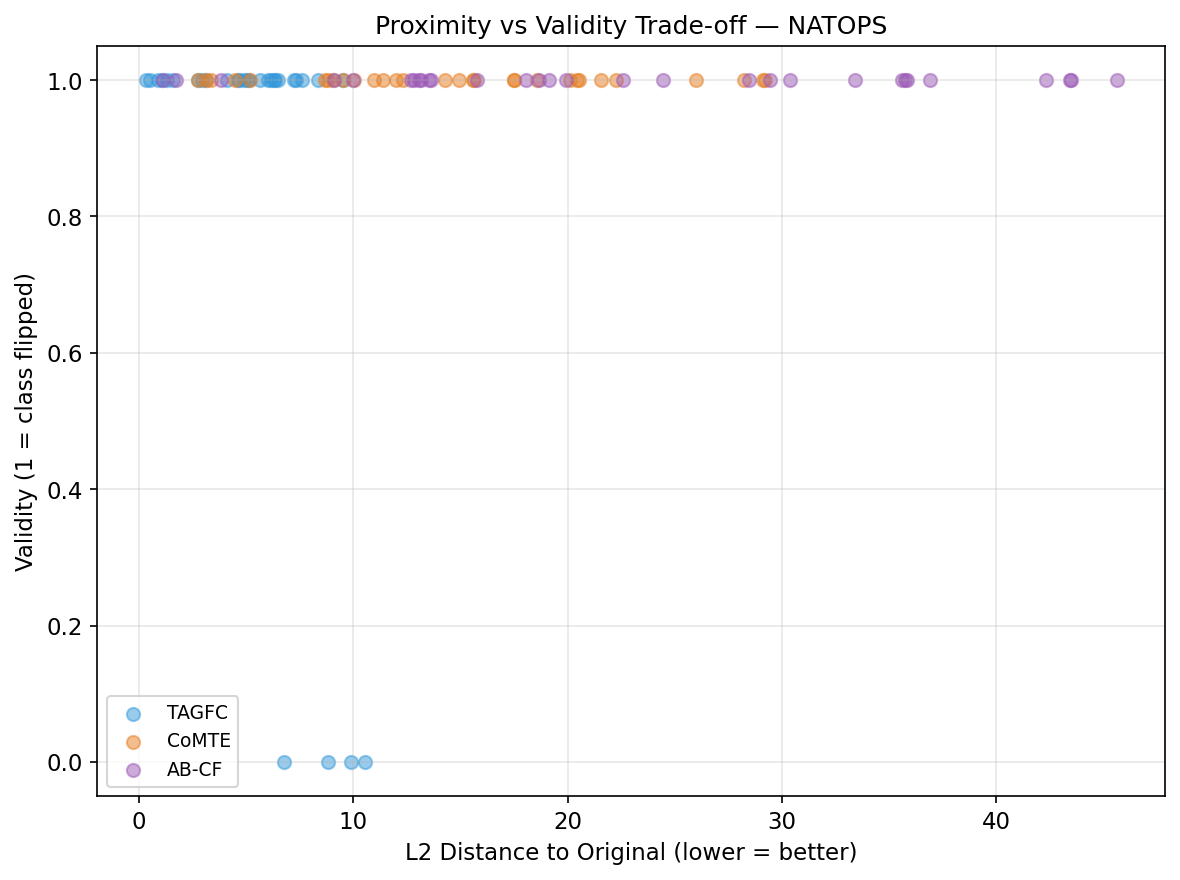
\includegraphics[width=0.85\textwidth]{../TAGFC_Natops/outputs/figures/F11_proximity_validity_scatter.png}
    \caption{NATOPS — Proximity ($L2$) vs.\ Validity scatter plot for TAGFC (blue), CoMTE (orange), and AB-CF (green). Valid counterfactuals ($y=1$) are shown at the top; invalid ($y=0$) at the bottom. TAGFC valid counterfactuals cluster at significantly lower $L2$ values than both baselines.}
    \label{fig:scatter}
\end{figure}

The scatter plot reveals two key observations:

\textbf{(1) TAGFC valid counterfactuals are significantly more compact.} Among valid instances (top row, $y=1$), TAGFC points cluster at $L2 \in [0.32, 10.55]$, while CoMTE valid points range up to $L2 \approx 29.2$ and AB-CF up to $L2 \approx 45.6$. This confirms that TAGFC's wavelet-domain optimisation finds genuinely closer paths to the decision boundary.

\textbf{(2) TAGFC invalid instances are rare but structured.} The 4 TAGFC invalid instances (bottom row, $y=0$) correspond to query instances where the NUN is particularly far from the query (high $\|\mathbf{X}^* - \mathbf{X}\|_F$), causing the manifold loss $\mathcal{L}_{\text{manifold}}$ to act as a strong anchor that prevents the flip loss from dominating. These edge cases can be resolved by increasing $\lambda_3^{-1}$ (reducing manifold anchoring) or the iteration budget.

\textbf{(3) AB-CF trades validity for proximity differently from TAGFC.} AB-CF achieves 100\% validity because its segment-swap approach guarantees a class flip at the cost of replacing large portions of the signal (high $L2$). TAGFC's 86.7\% validity with low $L2$ represents a fundamentally different operating point on the validity--proximity Pareto frontier: it generates more compact counterfactuals for the instances where it succeeds.

%========================================================================
\section{Summary of Findings}

Four principal findings emerge. TAGFC achieves statistically significant lower proximity ($L2$, $L\infty$; $p < 0.0001$) with effect sizes of $2.84\times$ vs CoMTE and $4.39\times$ vs AB-CF. Cross-sensor coherence is $5.7\times$–$5.8\times$ better than both baselines ($p < 0.0001$), validating the Mahalanobis penalty. TAGFC's RCF of 0.217 substantially outperforms CoMTE (0.647) and AB-CF (1.027); AB-CF's RCF $> 1$ exposes a fundamental failure of segment-swap methods for distant NUN pairs. Finally, time-domain sparsity is not the correct measure for wavelet-domain methods: TAGFC's near-zero score is an inverse-DWT artefact, while coefficient-level sparsity (guaranteed by soft-thresholding) is the appropriate measure.

\clearpage
\typeout{}
\chapter{Conclusion and Future Work}

%========================================================================
\section{Summary of Contributions}

This work presented \textbf{TAGFC} (Transformer Attention-Guided Frequency Counterfactual), a novel framework for generating actionable counterfactual explanations for Transformer-based multivariate time-series classifiers, evaluated on NASA CMAPSS FD001 and NATOPS against CoMTE and AB-CF using eight quantitative metrics and rigorous statistical testing.

Three unique contributions are made. \textbf{(1) Frequency-domain counterfactual generation}: TAGFC is the first method to perturb wavelet coefficients rather than raw time-domain values, producing frequency-localised, physically interpretable modifications — slow HPC drift in approximation coefficients, fast transients in detail coefficients — entirely absent from all prior work. \textbf{(2) Model-aware saliency via attention rollout}: by propagating multi-head self-attention through all $L$ layers and $H$ heads with residual weighting, TAGFC builds omega importance weights that focus perturbations on model-relevant timesteps, yielding more compact and interpretable counterfactuals than black-box or output-only baselines. \textbf{(3) Cross-sensor physical coherence}: the Mahalanobis penalty achieves coherence $5.7\times$--$5.8\times$ lower than both baselines ($p < 0.0001$), ensuring multi-sensor perturbations respect the physical covariance structure of real sensor data — a prerequisite for operationally actionable recommendations.

%========================================================================
\section{Limitations}

TAGFC has four notable limitations. \textbf{Validity gap}: the constrained four-term optimisation achieves 86.7\% validity on NATOPS (vs.\ 100\% for both baselines) because the manifold and sparsity losses may prevent convergence within the iteration budget — a fundamental tension between minimality and guaranteed flip. \textbf{Time-domain sparsity measurement}: near-zero time-domain sparsity is an inverse-DWT artefact, not a true reflection of coefficient-level sparsity, creating a metric mismatch when comparing against time-domain methods. \textbf{Haar wavelet assumption}: the piecewise-constant Haar basis suits CMAPSS's piecewise-linear degradation model but may be suboptimal for smooth signals; Daubechies or learned wavelets would generalise better. \textbf{NUN retrieval cost}: exhaustive $\mathcal{O}(NTD)$ search becomes a bottleneck for $N > 10^5$; approximate methods (e.g., FAISS) would address this.

%========================================================================
\section{Future Work}

Six high-priority directions are identified for future research.

\begin{enumerate}
    \item \textbf{Ablation study.} Systematically ablate each TAGFC component: (a) \textit{noRollout} — uniform omega weights; (b) \textit{noWavelet} — time-domain perturbation; (c) \textit{noCross} — $\lambda_2=0$; (d) \textit{noManifold} — $\lambda_3=0$, to quantify each component's independent contribution.

    \item \textbf{Extend to regression-based RUL prediction.} Replace the cross-entropy flip loss with a margin loss $\max(0, f(\widetilde{\mathbf{X}}) - \tau)$ for a target RUL threshold $\tau$, enabling counterfactual generation directly over continuous RUL outputs.

    \item \textbf{Apply to CMAPSS FD002--FD004 and additional UEA datasets.} FD002--FD004 introduce multiple operating conditions and fault modes; evaluating TAGFC on these and further UEA benchmarks would validate generalisation beyond single-condition settings.

    \item \textbf{Replace Haar with Daubechies or learned wavelets.} Smoother orthonormal wavelets (e.g., Daubechies-4, Symlet-4) would better model continuously varying dynamics; a learned dictionary could further adapt the basis per dataset.

    \item \textbf{Real-time counterfactual generation.} Amortised inference via a conditional VAE or normalising flow could replace iterative Proximal GD, reducing per-query runtime from seconds to milliseconds for online deployment.

    \item \textbf{Causal counterfactual generation.} Replacing the Mahalanobis coherence penalty with a structural causal model (SCM) constraint would guarantee that generated counterfactuals correspond to causally achievable system interventions.
\end{enumerate}

\typeout{}
\begin{thebibliography}{99}

\bibitem{lei2018machinery}
Y.~Lei, B.~Yang, X.~Jiang, F.~Jia, N.~Li, and A.~K. Nandi,
``Machinery health prognostics: A systematic review from data acquisition to rul prediction,''
\textit{Mechanical Systems and Signal Processing}, vol.~104, pp.~799--834, 2018.

\bibitem{fink2020prognostics}
O.~Fink, E.~Zio, and U.~Weidmann,
``Prognostics and health management---a review on data driven approaches,''
\textit{European Journal of Operational Research}, vol.~279, no.~3, pp.~774--794, 2020.

\bibitem{mckinsey2017}
McKinsey \& Company,
``The value of predictive maintenance,''
\texttt{https://www.mckinsey.com}, 2017.

\bibitem{mobley2019}
R.~K. Mobley,
\textit{An Introduction to Predictive Maintenance}.
Elsevier, 2019.

\bibitem{nectoux2012pronostia_a}
P.~Nectoux, R.~Gouriveau, K.~Medjaher, E.~Ramasso, B.~Morello, N.~Zerhouni, and C.~Varnier,
``Pronostia: An experimental platform for bearings accelerated degradation tests,''
in \textit{2012 IEEE International Conference on Prognostics and Health Management (PHM)}, 2012.

\bibitem{saxena2008damage}
A.~Saxena, K.~Goebel, D.~Simon, and N.~Eklund,
``Damage propagation modeling for aircraft engine run-to-failure simulation,''
in \textit{Proceedings of the 1st International Conference on Prognostics and Health Management (PHM'08)}, 2008.

\bibitem{guidotti2024counterfactual}
R.~Guidotti,
``Counterfactual explanations and how to find them: literature review and benchmarking,''
\textit{Data Mining and Knowledge Discovery}, vol.~38, no.~5, pp.~2770--2824, 2024.

\bibitem{lundberg2017unified}
S.~M. Lundberg and S.-I. Lee,
``A unified approach to interpreting model predictions,''
in \textit{Advances in Neural Information Processing Systems 30}, 2017.

\bibitem{ribeiro2016trust}
M.~T. Ribeiro, S.~Singh, and C.~Guestrin,
```Why should I trust you?': Explaining the predictions of any classifier,''
in \textit{Proceedings of the 22nd ACM SIGKDD}, 2016.

\bibitem{wachter2017counterfactual}
S.~Wachter, B.~Mittelstadt, and C.~Russell,
``Counterfactual explanations without opening the black box: Automated decisions and the GDPR,''
\textit{Harvard Journal of Law \& Technology}, vol.~31, no.~2, 2017.

\bibitem{mothilal2020explaining}
R.~K. Mothilal, A.~Sharma, and C.~Tan,
``Explaining machine learning classifiers through diverse counterfactual explanations,''
in \textit{Proceedings of the 2020 ACM Conference on Fairness, Accountability, and Transparency (FAT*)},
pp.~607--617, 2020.

\bibitem{jin2025tcntransformer}
X.~Jin, Y.~Ji, S.~Li, K.~Lv, J.~Xu, H.~Jiang, and S.~Fu,
``Remaining useful life prediction for rolling bearings based on TCN--Transformer networks using vibration signals,''
\textit{Sensors}, vol.~25, no.~11, p.~3571, 2025.

\bibitem{zhou2021transformer}
Z.~T. Zhou, L.~Liu, X.~Song, et~al.,
``Remaining useful life prediction method of rolling bearing based on Transformer model,''
\textit{Journal of Beijing University of Aeronautics and Astronautics}, vol.~49, no.~2, pp.~430--443, 2021.

\bibitem{zou2023multiscale}
W.~Zou, Z.~Lu, Z.~Hu, and L.~Mao,
``Remaining useful life estimation of bearing using deep multiscale window-based transformer,''
\textit{IEEE Transactions on Instrumentation and Measurement}, vol.~72, pp.~1--11, 2023.

\bibitem{moosavi2024explainable}
S.~Moosavi, M.~Farajzadeh-Zanjani, R.~Razavi-Far, V.~Palade, and M.~Saif,
``Explainable AI in manufacturing and industrial cyber--physical systems: A survey,''
\textit{Electronics}, vol.~13, no.~17, p.~3497, 2024.

\bibitem{li2022sgcf}
P.~Li, O.~Bahri, S.~Filali Boubrahimi, and S.~M. Hamdi,
``SG-CF: Shapelet-guided counterfactual explanation for time series classification,''
in \textit{2022 IEEE International Conference on Big Data (Big Data)}, pp.~1564--1573, 2022.

\bibitem{sanderson2025dipace}
J.~Sanderson, H.~Mao, and W.~L. Woo,
``DiPACE: Diverse, plausible and actionable counterfactual explanations,''
in \textit{Proceedings of the 17th International Conference on Agents and Artificial Intelligence (ICAART 2025)},
vol.~2, pp.~543--554, 2025.

\bibitem{ding2021convolutional}
Y.~Ding and M.~Jia,
``A convolutional Transformer architecture for remaining useful life estimation,''
in \textit{2021 Global Reliability and Prognostics and Health Management (PHM-Nanjing)},
pp.~1--6, 2021.

\bibitem{duan2024deepar}
Z.~Duan et~al.,
``Intelligent prediction of rolling bearing remaining useful life based on probabilistic DeepAR-Transformer model,''
\textit{Measurement Science and Technology}, vol.~35, no.~1, p.~015107, 2024.


\bibitem{ates2021counterfactual}
E.~Ates, B.~Aksar, V.~J. Leung, and A.~K. Coskun,
``Counterfactual explanations for multivariate time series,''
in \textit{Proceedings of the 2021 International Conference on Applied Artificial Intelligence (ICAPAI)},
pp.~1--8, 2021.
DOI: 10.1109/ICAPAI49758.2021.9462056.

\bibitem{li2023abcf}
P.~Li, O.~Bahri, S.~Filali Boubrahimi, and S.~M. Hamdi,
``Attention-based counterfactual explanation for multivariate time series,''
in \textit{International Conference on Big Data Analytics and Knowledge Discovery (DaWaK)},
pp.~315--329, 2023.
DOI: 10.1007/978-3-031-39831-5\_26.

\bibitem{delaney2021instance}
E.~Delaney, D.~Greene, and M.~T. Keane,
``Instance-based counterfactual explanations for time series classification,''
in \textit{Proceedings of the 29th International Conference on Case-Based Reasoning (ICCBR)},
2021. arXiv:2009.13211.

\bibitem{bahri2022sets}
O.~Bahri, P.~Li, S.~Filali Boubrahimi, and S.~M. Hamdi,
``Shapelet-based counterfactual explanations for multivariate time series,''
in \textit{KDD Workshop on Mining and Learning from Time Series (MiLeTS)},
2022. arXiv:2208.10462.

\bibitem{heimes2008recurrent}
F.~O. Heimes,
``Recurrent neural networks for remaining useful life estimation,''
in \textit{Proceedings of the 2008 International Conference on Prognostics and Health Management (PHM)},
Denver, CO, USA, 2008, pp.~1--6.

\bibitem{zhang2011extracting}
X.~Zhang and Y.~Zhao,
``Extracting key postures with sparse auto-encoder from motion capture data,''
in \textit{Proceedings of the 22nd British Machine Vision Conference (BMVC)}, 2011.

\bibitem{vaswani2017attention}
A.~Vaswani, N.~Shazeer, N.~Parmar, J.~Uszkoreit, L.~Jones, A.~N. Gomez, {\L}.~Kaiser, and I.~Polosukhin,
``Attention is all you need,''
in \textit{Advances in Neural Information Processing Systems 30 (NeurIPS)}, 2017, pp.~5998--6008.

\bibitem{zerveas2021transformer}
G.~Zerveas, S.~Jayaraman, D.~Patel, A.~Bhamidipaty, and C.~Eickhoff,
``A transformer-based framework for multivariate time series representation learning,''
in \textit{Proceedings of the 27th ACM SIGKDD Conference on Knowledge Discovery and Data Mining},
2021, pp.~2114--2124.

\bibitem{li2018remaining}
J.~Li, X.~Li, and D.~He,
``Remaining useful life estimation in prognostics using deep convolution neural networks,''
\textit{Reliability Engineering \& System Safety}, vol.~172, pp.~1--11, 2018.

\bibitem{cpcb2020aqi}
Central Pollution Control Board (CPCB),
``Air Quality Data --- \texttt{city\_day.csv},''
Kaggle, 2020.
\texttt{https://www.kaggle.com/datasets/rohanrao/air-quality-data-in-india}.

\bibitem{bagnall2018uea}
A.~Bagnall, H.~A. Dau, J.~Lines, M.~Flynn, J.~Large, A.~Bostrom, P.~Southam, and E.~Keogh,
``The UEA multivariate time series classification archive, 2018,''
arXiv:1811.00075, 2018.

\bibitem{loshchilov2019decoupled}
I.~Loshchilov and F.~Hutter,
``Decoupled weight decay regularization,''
in \textit{Proceedings of the 7th International Conference on Learning Representations (ICLR)}, 2019.

\bibitem{abnar2020quantifying}
S.~Abnar and W.~Zuidema,
``Quantifying attention flow in transformers,''
in \textit{Proceedings of the 58th Annual Meeting of the Association for Computational Linguistics (ACL)},
2020, pp.~4190--4197.

\end{thebibliography}

\typeout{}

% Bibliography is included via refrences.tex (thebibliography environment)

\end{document}
